\documentclass[11pt, a4paper, pdftex, twoside, dvipsnames]{article}
% font:
\usepackage{amsmath,amssymb,amsthm,amsfonts}
\usepackage{bm}  % From amsmath, a bold font
\newcommand{\argmax}{\mathop{\rm arg~max}\limits}
\newtheorem{them}{Theorem}
\newtheorem{prop}{Proposition}
\newtheorem{defn}{Definition}
\everymath{\displaystyle}
\allowdisplaybreaks
\usepackage{mathtools}
\usepackage[makeroom]{cancel}
%\usepackage{newtxtext,newtxmath}
\usepackage[title]{appendix}
\usepackage{epigraph}
% --------------------------------------------------------------------------- %
% figure:
\usepackage[labelfont=bf,font=small]{caption}
%\captionsetup[figure]{name=Fig.,labelsep=space}
%\captionsetup[table]{name=Table\ ,labelsep=space,font=normal}
%\usepackage{subfig}
% \subcaption with {}:
%\captionsetup{subrefformat=parens}
\usepackage{rotating}
\usepackage{float}
\usepackage{graphicx}  % remove 'demo' option for your real document
% --------------------------------------------------------------------------- %
% table


\usepackage{siunitx}


\usepackage{tabularx}
\usepackage{numprint}
\usepackage[dvipsnames]{xcolor}

\usepackage{xstring}


\sisetup{
%exponent-mode = engineering,
round-mode = places,
round-precision = 3
}


\usepackage{threeparttable}
\usepackage{multirow}
\usepackage{multicol}
\usepackage{blkarray}
\usepackage{booktabs}
\usepackage{arydshln}
\usepackage{tabularx}
\usepackage{longtable, array}
\newcolumntype{P}[1]{>{\raggedright\arraybackslash}p{#1}}
\usepackage{tikz}
\usetikzlibrary{arrows.meta}
%\usepackage[dvipsnames]{xcolor}
% --------------------------------------------------------------------------- %
% necessary usepackage
%\usepackage[x11names]{xcolor}
% Hyperref:
\usepackage[bookmarks=false, bookmarksnumbered=true,
colorlinks=true,setpagesize=false,
pdftitle={},pdfauthor={SimonScheidegger},pdfsubject={},
pdfkeywords={}, bookmarkstype=toc, urlcolor=black, citecolor=blue,
linkcolor=black, filecolor=black]{hyperref}


\hypersetup{
    colorlinks=true,
    linkcolor=red,
    filecolor=magenta,      
    urlcolor=cyan
    }


\usepackage{indentfirst}
% \setlength{\parindent}{0pt}
% \setlength{\parskip}{1ex plus 0.5ex minus 0.2ex} 
\usepackage{enumitem}
\usepackage{cases}
\usepackage{url}
\usepackage{setspace}
% \singlespacing
% \doublespacing
\setstretch{1}
\usepackage{ulem}
\usepackage{lscape}
\usepackage{here}
\usepackage{authblk}
\usepackage{framed}
\usepackage{adjustbox}
\usepackage{pdflscape}
\usepackage{listings}
\usepackage{cleveref}
\crefname{equation}{Eq.}{Eqs.}
\crefname{figure}{Figure}{Figures}
\crefname{table}{Table}{Tables}
\crefname{line}{Algorithm}{Algorithms}
\crefname{asmp}{Assumption}{Assumptions}
\crefname{section}{Section}{Sections}
\crefname{chapter}{Chapter}{Chapters}
\crefname{appsec}{Appendix}{Appendixes}
\let\normalref\ref
\renewcommand{\ref}{\cref}
%\usepackage{subcaption}
% \subcaption with {}:
%\captionsetup{subrefformat=parens}


\usepackage[bottom]{footmisc}

%%%%%%%%% Aryan's Macros %%%%%%%%
\DeclareFontFamily{U}{mathx}{}
\DeclareFontShape{U}{mathx}{m}{n}{<-> mathx10}{}
\DeclareSymbolFont{mathx}{U}{mathx}{m}{n}
\DeclareMathAccent{\widehat}{0}{mathx}{"70}
\DeclareMathAccent{\widecheck}{0}{mathx}{"71}
\newcommand{\too}[2]{\text{#1} \! \to \! \text{#2}}
\newcommand{\bb}[1]{\boldsymbol{\bold{#1}}}
\newcommand{\bbh}[1]{\widehat{\boldsymbol{\bold{#1}}}}
\newcommand{\bbb}[1]{\overline{\boldsymbol{\mathrm{#1}}}}
\newcommand{\bbt}[1]{\tilde{\boldsymbol{\mathrm{#1}}}}
\newcommand{\bbv}[1]{\text{vec}({\boldsymbol{\mathrm{#1}}})}
\newcommand{\ekk}[0]{\mathcal{K}}
\newcommand{\spn}[2]{ \text{span}\{#1 \,:\, #2 \}}
\newcommand{\card}[1]{|#1|}
\newcommand{\nnz}[1]{\text{nnz}(#1)}
\newcommand{\abs}[1]{\text{Abs}(#1) }
\newcommand{\maximize}[1]{\underset{ #1 }{\text{max}} }
\newcommand{\argmin}[1]{\underset{#1}{\text{argmin}} }
%\newcommand{\argmax}[1]{\underset{#1}{\text{arg~max}~} }
\newcommand{\minimize}[1]{\underset{ #1 }{\text{min}} }
\newcommand{\subjectTo}[0]{\text{s.t.}\quad }
\newcommand{\nn}{\newline\newline\noindent}
\newcommand{\sign}[1]{\text{sign}(#1)}
\newcommand{\tr}[1]{\text{tr}(#1)}
\newcommand{\ameq}[0]{\bb{a},\bbt{m}}
\newcommand{\expnum}[2]{
\ifnum#1=1 
  10^{#2} 
\else 
  #1 \! \cdot \! 10^{#2}
\fi
}

%%%%%%%%% Aryan's Macros %%%%%%%%




\newcommand{\fixmeAlex}[1]{\textbf{\emph{\textcolor{red}{/* TBD Alex: #1 */}}}}
\newcommand{\fixmeSimon}[1]{\textbf{\emph{\textcolor{blue}{/* TBD Simon: #1 */}}}}
\newcommand{\fixmeFelix}[1]{\textbf{\emph{\textcolor{red}{/* TBD Felix: #1 */}}}}
\newcommand{\fixmeDoris}[1]{\textbf{\emph{\textcolor{red}{/* TBD Doris: #1 */}}}}
\newcommand{\fixmeAryan}[1]{\textbf{\emph{\textcolor{red}{/* TBD Doris: #1 */}}}}
\newcommand{\Question}[1]{\textbf{\emph{\textcolor{red}{/* Question to all: #1 */}}}}

% --------------------------------------------------------------------------- %
% size of the paper: A4
\usepackage[a4paper,left=2cm,right=2cm,top=2.5cm,bottom=2.5cm]{geometry}
% setting for header
\usepackage{fancyhdr}
\pagestyle{fancy}
% \fancyhead[RO,LE]{\thepage}
% \fancyhead[RE,LO]{{\textsf \leftmark}}
% \fancyfoot{}
% \fancyhead[re,lo]{\sffamily\nouppercase{\leftmark}}
\fancyhead[re,lo]{}
\fancyhead[ro,le]{\thepage}
\fancyfoot{}
% for the first page
\fancypagestyle{firstpagestyle}{
\renewcommand{\headrulewidth}{0pt}
\fancyhf{} % clear all header and footer fields
\fancyfoot[C]{\thepage}
}
% for the first page of CV
\fancypagestyle{CVfirstpagestyle}{
\renewcommand{\headrulewidth}{0pt}
\fancyhf{} % clear all header and footer fields
\fancyfoot[C]{\thepage}
}
% --------------------------------------------------------------------------- %
% BibLaTeX with jecon bibliography style
\usepackage{natbib}
\bibliographystyle{jpe}
%-------------------------------------------
% Macros
\renewcommand{\vec}[1]{{\mathbf{#1}}}
\newcommand{\mat}[1]{\underline{\underline{\vec{#1}}}}

% --------------------------------------------------------------------------- %
% rename:
\renewcommand{\refname}{Bibliographies}
\renewcommand{\abstractname}{Abstract}
\newcommand{\defeq}{\mathrel{\mathop:}=}
\newcommand{\eqdef}{\mathrel{\mathop=}:}
\renewcommand{\topfraction}{1.0}
\renewcommand{\bottomfraction}{1.0}
\renewcommand{\dbltopfraction}{1.0}
\renewcommand{\textfraction}{0.01}
\renewcommand{\floatpagefraction}{1.0}
\renewcommand{\dblfloatpagefraction}{1.0}
\setcounter{topnumber}{5}
\setcounter{bottomnumber}{5}
\setcounter{totalnumber}{10}
% --------------------------------------------------------------------------- %
\title{Ocean, land, and atmosphere (OLA): a simple climate emulator for net-zero emission scenarios\thanks{We thank ..., as well as seminar participants at the University of Lausanne and the University of Zurich for very useful conversations and comments. This work was supported by the Swiss National Science Foundation (SNF), under project ID  \lq\lq Can Economic Policy Mitigate Climate-Change?\rq\rq, and for research support. Simon Scheidegger gratefully acknowledges support from the MIT Sloan School of Management.}}
\author{
    Aryan Eftekhari\thanks{TBA, UNI; Email:
    \href{mailto:bla}{bla.ch}.}, \;
    Pratyuksh Bansal\thanks{Institute of Computing, Universit\`a della Svizzera italiana; Email:
    \href{mailto:pratyuksh.bansal@sam.math.ethz.ch}{pratyuksh.bansal@sam.math.ethz.ch}.}, \;
    Doris Folini\thanks{Institute for Atmospheric and Climate Science, ETHZ; Email:
    \href{mailto:doris.folini@env.ethz.ch}{doris.folini@env.ethz.ch}.}, \;
  Felix K\"ubler\thanks{Department for Banking and Finance, University of Z\"urich; Swiss Finance Institute (SFI); Email: \href{mailto:fkubler@gmail.com}{felix.kuebler@bf.uzh.ch}.}, \\ \;
  Aleksandra Malova\thanks{Department of Economics, University of Lausanne; Email: \href{mailto:malova.alex@unil.ch}{aleksandra.malova@unil.ch}.}, \; 
  Simon Scheidegger\thanks{Department of Economics, University of Lausanne; Enterprise for Society (E4S); Email: \href{mailto:simon.scheidegger@unil.ch}{simon.scheidegger@unil.ch}}, \;
  Olaf Schenk\thanks{Institute of Computing, Universit\`a della Svizzera italiana; Email: \href{mailto:olaf.schenk@usi.ch}{olaf.schenk@usi.ch}.}
  }
\date{\today}

%pratyuksh.bansal
\begin{document}
\maketitle

\begin{abstract}
 We extend DICE-2016 with another time scale
 
 Wish list:
 \begin{itemize}
     \item Extreme econ cases to confront with different carbon cycles
 \end{itemize}

  \end{abstract}

{\small {\bf Keywords:} climate change, social cost of carbon, carbon taxes, environmental policy, deep learning, integrated assessment models, DICE-2016} \\

{\small {\bf JEL classification:} C61, E27, Q5, Q51, Q54, Q58} 



\newpage
% \tableofcontents

\newpage

%
%%%%%%%%%%%%%%%%%%%%%%%%%%%%%%%%%%%%%%%%%
\section{Introduction}
\label{sec:intro}
%%%%%%%%%%%%%%%%%%%%%%%%%%%%%%%%%%%%%%%%%
%
Suggested storyline:
\begin{itemize}
    \item 1 paragraph blabla
    \item motivations of current paper: point out of current DICE (e.g., RCP)
    \item on an abstract level: 1 dynamic timescale missing.
    \item on a concrete level. We cannot resolve e.g. RCP2.6
    \item What are the economic implications: aggressive mitigation cannot be handled, etc...
    \item contribution from our side: go from 3 to 4 or 5 reservoirs.
    \item show how to calibrate it. Extend also test set by more tests (CDICE) to pin down the additional degrees of freedom.
    \item Contribution to climate science as stand-alone (preview of results): with this simple model(s), we show that we can correctly capture a),b),c), which contradicts the present opinion in the literature.
    \item from an econ applications point of view, 
\end{itemize}



Climate modeling in the context of economic modeling consists, in essence, of translating carbon emissions generated by economic activity into atmospheric CO2 concentrations and on into a change in global mean temperature. Associated climate emulators (CEs) need to be computationally cheap, to free resources for the modeling of any none-climate aspects, yet 'fit for purpose~\footnote{See Folini et al. (2022) for a more detailed discussion of what is meant by 'fit for purpose'.}. The pivotal role of equilibrium climate sensitivity (ECS) when calculating the temperature change arising from an increase in atmospheric CO2 has long been recognized. A plausible reason why ECS has attracted so much attention from the economic community may be the uncertainty of ECS from a climate science point of view. Best estimates for ECS still range from roughly 2 to 4 degree Celsius, thus cannot be simply ignored in an economic context. Comparatively less attention is paid to uncertainties associated with the carbon-cycle, the second pillar of any climate model used in an economic context. Associated models vary in their level of complexity, ranging from simple impulse response function or two layer box models to more comprehensive models designed, for example, to account for hemispheric and depth dependent aspects of the oceans and to capture aspects of the land biosphere. The performance of one such model, a three-reservoir carbon-cycle model as used in the seminal DICE model, was assessed in some detail by Folini et al. (2022) from a climate science point of view and with regard to the impact of the carbon-cycle on economic aspects. It was demonstrated that i) a correct calibration of the carbon-cycle with respect to climate science bench marks is crucial and that ii) varying model calibration within bounds justified by climate science has a relevant impacts on economics, about half as big as from varying ECS (see Figure 12a in Folini et al. (2022)). The paper further stressed the relevance of the three-box carbon-cycle model featuring two response time scales, a fast and a slow one, in order to properly translate carbon emissions into atmospheric CO2 concentrations. 

The present paper is a follow-up on Folini et al. (2022) in that it addresses the question of whether adding more carbon reservoirs has a relevant effect on the performance of the CE with regard to climate science and economics. We examine models consisting of three, four, or five carbon reservoirs that represent the atmosphere, the ocean, and possibly the biosphere on land. Addition of a land biosphere reservoir also paves the way to study climate mitigation scenarios explicitly involving the land biosphere for carbon capture and storage. The later question is of relevance in view of the Paris agreement and associated climate targets, like the 1.5 degree target. Climate science claims that reaching these goals implies a rapid decline in emission and even negative emissions later in this century. The question arises whether simple carbon-cycle models as studied here are fit to purpose in view of such scenarios. 

Mitigation scenarios distinguish themselves from business as usual scenarios in that carbon emissions decrease or even become negative (carbon sequestration) instead of steadily growing. From a carbon-cycle point of view this implies that partial pressure differences between notably the atmosphere and the ocean become smaller with time, as carbon emissions to the atmosphere diminish. With the difference in CO2 partial pressure between atmosphere and ocean diminishing, the uptake efficiency of the ocean decreases. Under extreme scenarios, the ocean may even turn from a CO2 sink to a CO2 source. Modeling of such behavior, of such re-distribution of carbon among reservoirs, necessitates that the entity of emitted carbon over time is still present in the model. This is the case for carbon-cycle box models, but not necessarily for impulse response function models. We quantify the capability of the simple box models at the heart of this study to successfully emulate this behavior, making the models suitable to study the connection between economy, strong mitigation scenarios, and climate. 

We start from the functional form of the carbon-cycle as used in the widely used DICE-2016 model, a three-box model with one box for the atmosphere and two boxes for the ocean, one for the upper-ocean one for the deep-ocean. We add more reservoirs to the carbon-cycle model and follow the strategy outlined in Folini et al. (2022) to calibrate and bench mark the model. We note already here that additional bench marks specifically tailored to negative emissions or the land-biosphere reservoir do not form part of this study and are the topic of future work. Finally, we apply the newly calibrated carbon-cycle models to examine optimal abatement policies, focusing on whether the additional carbon-reservoirs make any difference in this resepect. 
The paper is organized as follows.


%We illustrate that this functional form is too simplistic to account for rapidly declining carbon emissions, thus is not fit for purpose if it comes to examine strong mitigation scenarios. We demonstrate that the addition of only one more reservoir, either representing a middle-ocean or the land-biosphere, substantially improve the performance. The added value of a five box model - atmosphere, land, upper, middle, and deep-ocean - is discussed. In summary, we argue that i) a carbon-cycle box model that is (carbon) mass preserving is compelling to study strong mitigation scenarios, that ii) at least a four box model is needed to reproduce key aspects of comprehensive climate model simulations, and that iii) only a five box model allows for examining the relative roles of ocean and land in future mitigation / negative emission scenarios.

%To this end, we first examine the behaviour of three, four, and five box carbon-cycle models for a standardised test case, the emission of 100 GtC to the present day atmosphere. We proceed with another idealized test case, where carbon emissions instantaneously are set to zero and inspect how the climate system and especially the temperature relaxes. The next logical step consists in examining the response not to a positive but to a negative emission pulse of 100 GtC, mimicking the instantaneous sequestration of carbon. Finally, we use the different carbon-cycle models in a realistic, strong mitigation setting. On the one hand via prescribing emissions, on the other hand via coupling the climate model to its economic counter part, asking for optimim mitigation.

%Maybe to the discussion? Here just some points from the literature, to be embedded in the text...\citet{macdougall-et-al:20} elaborate on what happens if emissions go instantaneously to zero. \citet{zickfeld-et-al:21} examine the asymmetry in climate response depending whether a positive carbon pulse (say 100 GtC) is injected to the atmosphere or whether instantaneously a certain amount of carbon (say 100 GtC) is removed from the atmosphere. The changing efficiency of ocean carbon uptake is the topic of \citet{ridge-mckinely:21}, with basic physics explained in \citet{raupach-et-al:14}. For negative emissions in DICE, see for example \citet{rickels-et-al:18}.


Things to stay before section 2
\begin{itemize}
	\item Pre-industrial is assume do 1765
	\item Carbon REservoires at pre-industrial times are based on \url{https://www.ipcc.ch/site/assets/uploads/2018/02/WG1AR5_Chapter06_FINAL.pdf}   
\end{itemize}


\begin{itemize}
	\item Stability: Reduces variability in parameter estimates for different benchmark. 
	\item short-time dynamics Salient 
	\item  Short-Term absorption discrepancy.      
\end{itemize}               


%%%%%%%%%%%%%%%%%%%%%%%%%%%%%%%%%%%%%%%%%%%%%%%
\newpage
\section{Climate Emulator}\label{sec:clim_model}
%%%%%%%%%%%%%%%%%%%%%%%%%%%%%%%%%%%%%%%%%%%%%%%
In this section, we will present our proposed methodology for a climate emulator, namely the carbon-cycle model, estimation procedure and calibration. 
%
We propose two carbon-cycle model configurations, which use serial and parallel reservoir configurations. 
The models we considered include three reservoir classes: atmosphere ($\text{A}$), ocean ($\text{O}$), and land-biosphere ($\text{L}$).
%
In the serial model, labeled as $3$SR, the carbon cycle is modeled as three sequentially connected carbon reservoirs, with the atmosphere connected to the upper ocean $\text{O}_1$, and the ocean connected to the deep ocean $\text{O}_2$. 
%
The parallel model labels  $4$PR,  introduces the land-biosphere, where carbon from the atmosphere is divided into two parallel streams: land-biosphere and ocean. 
%
The $4$PR model is an extension of $3$SR model by adding a single land biosphere reservoir ($\text{L}$); see, Figure~\ref{fig:1} for visualization.
\newline [more text]
\newline [more text]

%%%%%%%%%%%%%%%%%%%%%%%%%%%%%%%%%%%%%%%%%%%%%%%
\subsection{Carbon-Cycle}\label{sec:carbon_cycle}
%%%%%%%%%%%%%%%%%%%%%%%%%%%%%%%%%%%%%%%%%%%%%%%
Let $\bb{m}^t \in \mathbb{R}^{n}$ be the amounts of carbon in $p$ distinct reservoirs at discrete time steps $t = 1, 2, \ldots, T$. 
The carbon-cycle model can be characterized by the time-invariant operator $\bb{A} \in \mathbb{R}^{n \times n}$, which determines the rate of carbon mass exchange between these reservoirs. 
Accounting for emissions, denoted by $\bb{e}^t \in \mathbb{R}^{n}$, we describe the carbon-cycle using a first-order system of difference equations
%
\begin{align} \label{eq:clim_model.1}
    \bb{m}^t -\bb{m}^{t-1}  = \bb{A}\bb{m}^t +\bb{e}^{t},
\end{align}
%
where, $h$ is the time-step size, and where $\bb{m}^{0}$ is the \textit{initial condition}, which is known.
Throughout this paper we assume $h=1$.
The operator $\bb{A}$ possess real eigenvalues $-1 < \bb{\lambda}_i(\bb{A}) \leqslant 0$ for all $i$. 
For $i$ and $j$, there exists a carbon transfer path between the reservoirs if $\mathbf{A}_{ij} \neq 0$, and there is no carbon transfer path if $\mathbf{A}_{ij}=0$.
Furthermore, $\bb{A}$ is restricted to satisfy both the \emph{equilibrium condition} and the system \emph{mass conservation}. 
The equilibrium conditions of the carbon-cycle are defined as
%
\begin{align}\label{eq:clim_model.2}
    \bb{A}\bbt{m}=\bb{0},
\end{align}
%
where $\bbt{m}$ denotes the equilibrium carbon masses, which is proportional to the eigenvector associated with the zero eigenvalue of $\bb{A}$. 
The principle of mass conservation is upheld by ensuring that
%
\begin{align}\label{eq:clim_model.3}
    \bb{1}^\top (\bb{m}^{t}-\bb{m}^{t-1})= \bb{e}^{t}\; \forall \; t \iff \bb{1}^\top \bb{A} =\bb{0}.
\end{align}
%
We define the \textit{dynamic timescales} of the operator as $\bb{\tau}_i = 1/|\bb{\lambda}_i|$, excluding the zero eigenvalue, which corresponds to the infinite timescale associated with the equilibrium condition. 
Consequently, the potential dynamic timescales for the linear carbon-cycle model are $\bb{\tau}_i \in (1,\infty)$. 

\begin{figure}[b] 
\noindent\begin{minipage}[t]{0.4\linewidth}%
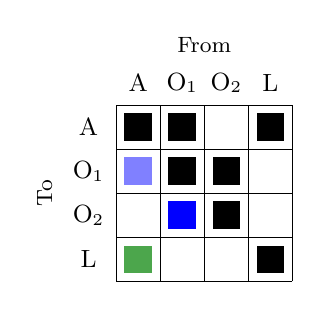
\begin{tikzpicture}
	\begin{scope}[shift={(0,0)},scale=.7]
        \node  at (1.6,5.1) {\footnotesize{From}}; 	
		\node  at (0.4,4.4) {\small$\text{A}$};
		\node  at (1.2,4.4) {\small$\text{O}_1$}; 
		\node  at (2.0,4.4) {\small$\text{O}_2$};
		 
		\node  at (2.8,4.4) {\small$\text{L}$}; 	
		%\node  at (3.6,4.4) {\small$\text{L}_2$}; 

        \node[rotate=90]  at (-1.3,2.4) {\footnotesize{To}}; 	
		\node  at (-0.5,3.6) {\small$\text{A}$}; 
		\node  at (-0.5,2.8) {\small$\text{O}_1$}; 
  	    \node  at (-0.5,2.0) {\small$\text{O}_2$};
  	     	
		\node  at (-0.5,1.2) {\small$\text{L}$};
		%\node  at (-0.5,0.4) {\small$\text{L}_2$}; 


		\node[fill=black,scale=1.5] at (0.4,3.6) (description) {};
		\node[fill=black,scale=1.5] at (1.2,3.6) (description) {};
		\node[fill=black,scale=1.5] at (2.8,3.6) (description) {};
  
		\node[fill=blue!50 ,scale=1.5] at (0.4,2.8) (description) {};
		\node[fill=black   ,scale=1.5] at (1.2,2.8) (description) {};
		\node[fill=black   ,scale=1.5] at (2.0,2.8) (description) {};
  
		\node[fill=blue!100 ,scale=1.5] at (1.2,2.0) (description) {};
		\node[fill=black    ,scale=1.5] at (2.0,2.0) (description) {};
		%\node[fill=black   ,scale=1.5] at (2.8,2.0) (description) {};
  
		\node[fill=black     ,scale=1.5] at (2.0,2.0) (description) {};
		%\node[fill=black    ,scale=1.5] at (2.8,2.0) (description) {};

		\node[fill=Green!70 ,scale=1.5] at (0.4,1.2) (description) {};
		\node[fill=black    ,scale=1.5] at (2.8,1.2) (description) {};
		%\node[fill=black   ,scale=1.5] at (3.6,1.2) (description) {};
  
  		%\node[fill=Green!100 ,scale=1.5] at (2.8,0.4) (description) {};
  		%\node[fill=black     ,scale=1.5] at (3.6,0.4) (description) {};
    	%\node[fill=black     ,scale=1.5] at (4.4,1.2) (description) {};


        \draw[step=.8, black] (0,.8) grid (3.2,4);  
        %\draw[black,very thick] (0,0) rectangle (3,3); 
	\end{scope}
\end{tikzpicture}
\end{minipage}
\noindent\begin{minipage}[t]{0.4\linewidth}%
\centering
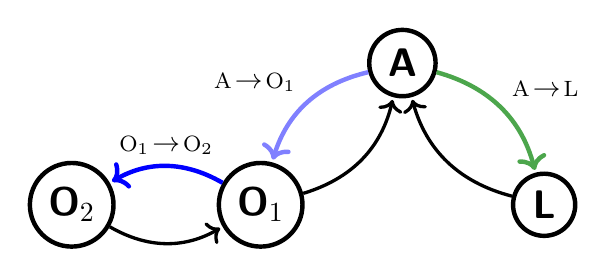
\begin{tikzpicture}[scale=0.6,->,shorten >=1pt,auto,
                        ultra thick,main node/.style={circle,draw,font=\sffamily\Large\bfseries}]
      \node[main node] (A) at (0,0) {A};
      \node[main node] (O1) at (-3,-3) {$\text{O}_1$};
      \node[main node] (O2) at (-7,-3) {$\text{O}_2$};
      \node[main node] (L1) at (3,-3) {$\text{L}$ };
     % \node[main node] (L2) at (7,-3) {$\text{L}_2$ };

\begin{scope}[ 
    shorten > = 1pt,
node distance = 3cm and 4cm,
    el/.style = {inner sep=2pt, align=left, sloped},
every label/.append style = {font=\tiny}      ]
      \path[->,ultra thick,blue!50] (A) edge [bend right] node [above left] {$\color{black}{\footnotesize{\too{A}{$\text{O}_1$}}}$} (O1);
      \path[->,very thick] (O1) edge [bend right] node [left] {} (A);      
    %
    \path[->,ultra thick,Green!70] (A) edge [bend left] node [above right]  {$\color{black}{\footnotesize{\too{A}{$\text{L}$}}}$} (L1);
    \path[->,very thick] (L1) edge [bend left] node [right] {} (A);
    %
    %\path[->,ultra thick,Green!100] (L1) edge [bend left] node [above]  {$\color{black}{\footnotesize{\too{$\text{L}_1$}{$\text{L}_2$}}}$} (L2);
    %  \path[->,very thick] (L2) edge [bend left] node [right] {} (L1);

      \path[->,ultra thick,blue!100] (O1) edge [bend right] node [above]  {$\color{black}{\footnotesize{\too{$\text{O}_1$}{$\text{O}_2$}}}$} (O2);
      \path[->,very thick] (O2) edge [bend right] node [above] {} (O1);

    \end{scope}
    \end{tikzpicture}
\end{minipage}
\caption{
The operator $\bb{A}$ is visualized (left) for the $4$PR model, which includes atmosphere ($\text{A}$), two ocean  reservoirs($\text{O}_1$ and $\text{O}_2$), and a land reservoirs ($\text{L}$). A graphically representation of the connectivity of the reservoirs (right) is shown with the unknown carbon mass transfer rates denoted, for example, $\text{O}_1 \! \to  \! \text{O}_2$ corresponds to the entry $\bb{A}_{3,2}$. The $3$SR model is a can all be considered as subsets of the more complex $4$PR model configuration. $\bb{A}$ is symmetric in its nonzero pattern, but not in its values.
}
\label{fig:1}
\end{figure}


Denote the nonzero strictly lower-triangular indices of $\bb{A}$ as $\mathcal{I}:=\{(i,j):\bb{A}_{ij}\neq 0,i>j\}$.
%
For all model configurations outlined, the closed-form solutions for the upper triangular values of the operator satisfying both \eqref{eq:clim_model.2} and \eqref{eq:clim_model.3} is
%
\begin{align} \label{eq:clim_model.4}
	\bb{A}_{ji} = \bb{A}_{ij}  \frac{\bbt{m}_j}{\bbt{m}_i} \; \forall \; (i,j) \in \mathcal{I}, \; \text{and} \;  \bb{A}_{ii}= -\sum_{j=1,j\neq i}^p \bb{A}_{ij}.
\end{align}
%
The necessary \emph{admissible parameters} required to define the operator include the strictly lower triangular nonzero values $\bb{a}:=\{ \bb{A}_{ij}: (i,j) \in \mathcal{I} \}$ and the equilibrium masses $\bbt{m}$, for which the parameterized operator, denoted as $\bb{A}[\ameq]$ has eigenvalues satisfying $-1 < \bb{\lambda}_i(\bb{A}[\ameq]) \leqslant 0$.
%
For a predefined sequence of emissions $\bb{E}:=(\bb{e}^{1},\bb{e}^{2},\ldots,\bb{e}^T)$ of length $T$ the carbon-cycle simulation denoted as    
%
\begin{align} \label{eq:clim_model.5}
	\bb{M}[\ameq] := (\bb{m}^{1},\bb{m}^{2},\ldots,\bb{m}^{T} ), 
\end{align}
%
where $\bb{m}^{t}$ is defined as per \eqref{eq:clim_model.1}. 
%
We utilize acronyms depicted in Figure~\ref{fig:1} to refer to specific reservoirs; for instance, $\bb{M}[\ameq]^{t}_{\text{O}_2}=\bb{m}^t_{\text{O}_2}$ represents the content of the $\text{O}_2$ or deep-ocean reservoir at time $t$.
%
Throughout this section, our simulations are exclusively use atmospheric emissions, meaning $\bb{e}_{\text{A}}^t$ is nonzero only when emissions are present at time $t$, while all other entries are zero.
%The time stepping scheme used for the carbon-cycle simulation is implicit Euler. 
%
%By simplifying the problem and setting $\bb{m}^{\text{eq}}$ to the preindustrial values found in Table~\ref{tab:1} (see, e.g.,~\cite{2431585063dd4b78b890f885bb19642e} and reference therein for further details), we reduce the unknown parameters to the nonzero values in the strictly lower-triangular matrix $\bb{A}$ (as seen in Figure~\ref{eq:clim_model.1}). 
%
%For the given model configurations, this corresponds to $n-1$ parameters.
%
%%%%%%%%%%%%%%%%%%%%%%%%%%%%%%%%%%%%%%%%%%%%%%%
\subsection{Fitting Procedure} \label{sec:2.2}
%%%%%%%%%%%%%%%%%%%%%%%%%%%%%%%%%%%%%%%%%%%%%%%
\begin{figure}[t]
    \centering
    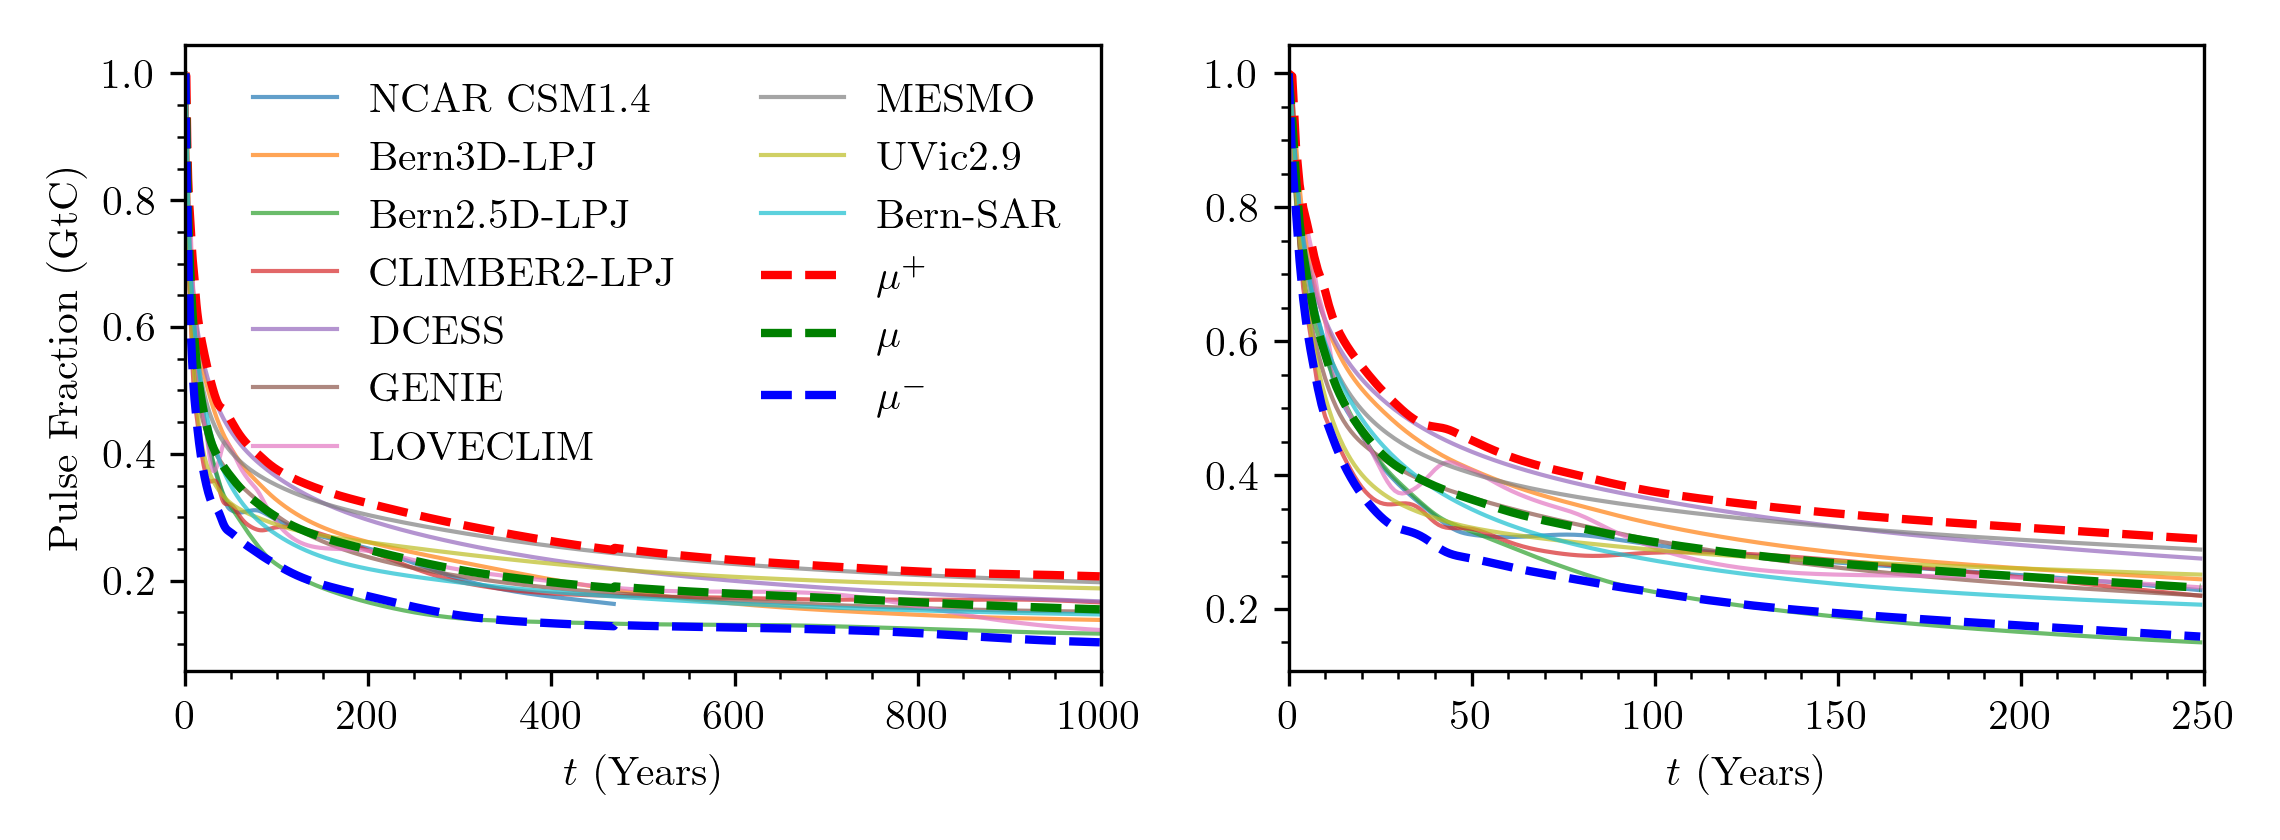
\includegraphics[width=\textwidth]{fig/solver_pulse.png}
    \caption{
    The decay of a $100$ GtC pulse of emissions in the pre-industrial atmosphere (1765) was analyzed using various Earth System Models of differing complexities.
    This data is based on a series of controlled simulations conducted by~\cite{joos2013carbon}.
    %For further details on the simulations and model descriptions, we refer the reader to the cited reference. T
    The multimodal mean of the simulations, denoted by $\mu$, along with the two standard deviations above and below $\mu$-benchmark, are represented by $\mu^+$ and $\mu^-$, respectively.
     }
    \label{fig:2}
\end{figure}
%

The proposed linear carbon-cycle is a simplified approximation of a considerably more complex system; our goal here to fit the model parameters for the $3$SR and $4$PR model configuration, such that we capture the salient dynamics of the carbon-cycle.
%
The proposed parameter fitting procedure aims to capture the pulse decay dynamics using a two-step process: first, we optimize the model parameters to emulate mean atmospheric pulse decay trajectory of a selected benchmarks; second, we present an approach to scale the fitted model to capture the extrema benchmarks of various benchmarks.
%
The simulation benchmarks introduced by~\cite{joos2013carbon}, and depicted in Figure~\ref{fig:1}, are use for the parameter fitting procedure. 
%
The benchmarks represent the atmospheric CO2 decay trajectories of a $100$ GtC pulse in various Earth System Models conducted in pre-industrial conditions in which the carbon-cycle is assumed to be at equilibrium.\footnote{See \url{https://climatehomes.unibe.ch/~joos/IRF_Intercomparison/results.html} for further details.}

%%%%%%%%%%%%%%%%%%%%%%%%%%%%%%%%%%%%%%%%%%%%%%%
\subsubsection{Mean parameter fitting} \label{sec:2.2.1}
%%%%%%%%%%%%%%%%%%%%%%%%%%%%%%%%%%%%%%%%%%%%%%%
We fit the operator parameters $\bb{a}$ and $\bbt{m}$ to best emulate the atmospheric CO2 masses after a $100$ GtC pulse.
%
The benchmark used in the fitting procedure is the multimodal mean of the various decay trajectories, which is referred to as the $\mu$-benchmark; see, Figure~\ref{fig:1} for visualization.
%
Specifically, we aim to minimize the discrepancy between the simulated atmospheric CO2 masses and those of the $\mu$-benchmark, while simultaneously imposing penalties on solutions that fail to align with observed carbon cycle attributes.
%
These attributes are encoded via penalty functions $q_1$, $q_2$ and $q_3$, which related to (i) dynamic time-scales, (ii) variability in equilibrium masses, and (iii) reservoir absorption ratios, respectively.
%
We will discuss the penalty functions in detail the paragraphs to follow.
%
Let $\bb{y}^{\mu} \in \mathbb{R}^{T}$ denote the atmospheric decay trajectory for the $\mu$-benchmark for $T$ years after the introduction of the $100$ GtC pulse.
%
 Given the non-negative tuning coefficients $\rho_1$, $\rho_2$, and $\rho_3$, each which correspond to the respective penalty functions, the $\mu$-benchmark fitted parameters are
 %
 \begin{align}\label{eq:obj}
 	\Big \{\bb{a}^{\mu},\bbt{m}^{\mu} \Big \} = \argmin{\{ \bb{a} , \bbt{m} \}}  
 	\Bigg\{  
 	     \frac{1}{T} \Big \| \bb{M}[\ameq]_\text{A} - \bb{y}^\mu \Big \|_2 +
 	 	 \rho_1 q_1(\ameq)   +  
 		 \rho_2 q_2(\bbt{m}) +   
 		 \rho_3 q_3(\ameq)  
 	\Bigg\}.
 \end{align}
%
Note that the model fit error with respect to the $\mu$-benchmark, appearing as the first term in the above objective function, relates solely to atmospheric masses; the masses of other reservoirs are controlled through the penalty terms.
%
Typically, we aim to minimize~\eqref{eq:obj} so that we can accurately emulate relatively short time-frames; that is to say, for $T$ is not so large. 
%
In our tests we use $T=250$ aligning with the time scales associated with the carbon exchange between the atmosphere and the Earth's surface, which span years to centuries.
%
%The dynamics further into the future carry much higher uncertainty and are less impactful to current decision-making policies and significance (see, e.g., Section~\ref{sec:econ} for further details).
%
%The transfer of carbon between the atmosphere and the Earth's surface occurs over time spans that range from years to centuries. The fit error model parameters to align with these temporal scales, aiming to closely approximate the µ-benchmark outlined in Equation \eqref{eq:obj}.

%%%%%%%%%%%%%%%%%%%%%%%%%%%%%%%%%%%%%%%%%%%%%%%
\paragraph{Dynamic time-scales:}
%%%%%%%%%%%%%%%%%%%%%%%%%%%%%%%%%%%%%%%%%%%%%%%
In addition to the carbon exchange between the atmosphere and the Earth's surface, we also take into account the long-term carbon cycles in deep soils and the deep ocean. 
%
These cycles occur over time frames ranging from centuries to millennia. 
%
To better mimic these carbon-cycle processes--especially those extending over longer dynamical time scales--the objective function~\eqref{eq:obj} incorporates the penalty function 
%
\begin{align}\label{eq:q1}
	q_1(\ameq) := -\frac{1}{n} \tr{\bb{A}[\ameq]} = -\frac{1}{n}\sum_{i=1}^n \bb{\lambda}_i(\bb{A}[\ameq]).
\end{align}
%\
This modification effectively biases the optimization program to favor operators $\bb{A}[\bb{a}, \bbt{m}]$ characterized by smaller average eigenvalues, or equivalently, by larger average time scales.
%
It is important to note that for all admissible parameters $\bb{a}$ and $\bbt{m}$, $q_1$ is strictly-positive. 


%%%%%%%%%%%%%%%%%%%%%%%%%%%%%%%%%%%%%%%%%%%%%%%
\paragraph{Equilibrium mass variability:}
%%%%%%%%%%%%%%%%%%%%%%%%%%%%%%%%%%%%%%%%%%%%%%%
The optimization problem in~\eqref{eq:obj} is not convex; this is clearly seen in~\eqref{eq:clim_model.4}, were only the ratios of $\bbt{m}$ are relevant; this implies that the fitted parameter $\bbt{m}$ is equivalent to $c\bbt{m}$ for any $c$.
%
As a result we can expect a high-degree of variability in the in the fitted parameter $\bb{a}$ and or $\bbt{m}$.
%
To reduce variability in the fitted parameters, we induce a bias in the objective to ensure that $\bbt{m}$ aligns with existing estimates of Earth's pre-industrial carbon reservoirs masses.
%
Let $\bbt{m}^*$ denote the estimated reservoir equilibrium masses.
%
We penalize the relative difference of $\bbt{m}$ with respect to $\bbt{m}^*$  using the penalty function  
%
\begin{align}\label{eq:q2}
	q_2(\bbt{m}) := \frac{1}{n} \Big\| (\bbt{m} - \bbt{m}^*) \oslash \bbt{m}^* \Big\|_2.
\end{align}
%
where $\oslash$ denote the elements-wise division. 
%
In our tests, $\bbt{m}^*$ is defined based one pre-industrial estimates outlined in~\cite{IPCC_carbon_cycle} where the reservoir equilibrium masses for the atmosphere, upper ocean, lower ocean, and land biosphere are $589$, $900$, $37\,100$, and $550$ GtC, respectively.

%%%%%%%%%%%%%%%%%%%%%%%%%%%%%%%%%%%%%%%%%%%%%%%
\paragraph{Reservoir absorption ratios:}
%%%%%%%%%%%%%%%%%%%%%%%%%%%%%%%%%%%%%%%%%%%%%%
Cumulative fluxes of carbon from the atmosphere to the ocean and land biosphere reservoirs significantly influence the overall response characteristics of the emulator. 
%
For instance, in the context of the $100$ GtC pulse, it is plausible that the $4$PR configuration could achieve a good fit for the atmospheric decay trajectory while maintaining minimal cumulative flux in the reservoir associated with land biosphere---essentially mimicking the behavior of the $3$SR model which lacks a land biosphere reservoir (see, e.g., Section~\ref{sec:2.1} for further details).
%
To ensure that the model mirrors the observed dynamics in the more complex Earth System Model (ESM), we enforce the ratios of cumulative ocean and land biosphere fluxes, denoted as $\eta$, at specific time period following the emission at $t_e$.
%
To approximate the cumulative ocean and land-biosphere flux ratio as $\eta$ at time $t_e$, deviations from this value is penalized using the penalty function
%
\begin{align}\label{eq:q3}
	q_3(\ameq) := \left \| \frac{  
	\bb{M}[ \ameq ]_{\text{O}}^{t_e}
	}{
	\bb{M}[ \ameq]_{\text{L}}^{t_e}} - \eta \right \|_2,
\end{align}
%
where $\bb{M}[\bb{A}]^{t_e}_{\text{O}}$ is the total mass of all ocean reservoirs (and similarly, the superscript $\text{L}$ denotes all land biosphere reservoirs).
%
We adopt the findings of~\cite{joos2013carbon}, whose experiments show that an equal $30$ GtC distribution between ocean and land-biosphere reservoirs is achieved, corresponding to $\eta = 1$, at $t_e = 20$ years after a $100$ GtC atmospheric pulse.
%
These are average values, for which any individual ESM may have differing values.


%%%%%%%%%%%%%%%%%%%%%%%%%%%%%%%%%%%%%%%%%%%%%%%
\subsubsection{Extrema parameter fitting} \label{sec:2.2.2}
%%%%%%%%%%%%%%%%%%%%%%%%%%%%%%%%%%%%%%%%%%%%%%%
As illustrated in Figure~\ref{fig:2}, various ESMs demonstrate different rates of $100$ GtC pulse decay trajectories. 
%
Here we aim to capture the extrema of these trajectories across different ESMs (see, e.g., Figure~\ref{fig:2}).
%
Similar to the mean fitting procedure outlined in the preceding section, these dynamics are not intrinsically linked to any particular ESM; rather, they define the plausible upper and lower limits for atmospheric carbon content during such a pulse event.
%
The proposed approach aims augmenting the fitted operator outlined in the previous section to represent two standard deviations above and below the $\mu$-benchmark, denoted as $\mu^+$ and $\mu^-$-benchmark, respectively.

Let $c^{\mu^-}\!\!\!, c^{\mu^+}\!\!\! \in \mathbb{R}^+$ be positive coefficients, corresponding to the $\mu^+$ and $\mu^-$-benchmark decay trajectories, respectively.
%
For $\bb{A}^{\mu}\!\!:=\bb{A}[\bb{a}^\mu,\bbt{m}^\mu]$, we represent the respective extrema operators  as $\bb{A}^{\mu^+}\!\!\!:= c^{\mu^+}\!\! \cdot \bb{A}^{\mu}$ and $\bb{A}^{\mu^-}\!\!\!:= c^{\mu^-}\!\! \cdot \bb{A}^{\mu}$.
%
Given the pulse decay trajectories $\bb{y}^{\mu^+}\!\!\!, \bb{y}^{\mu^-}\!\!\!  \in \mathbb{R}^T$,  with
%
\begin{align}\label{eq:objc}
  c^{\mu^+} \!= \argmin{c} \Bigg\{  \frac{1}{T}  \Big \| \bb{M}[c \cdot \bb{a}^\mu, \bbt{m}^{\mu}]_\text{A} - \bb{y}^{\mu^+} \Big \|_2  \Bigg\},\; \text{and} \; 
  c^{\mu^-} \!= \argmin{c} \Bigg\{  \frac{1}{T} \Big \| \bb{M}[c \cdot \bb{a}^\mu, \bbt{m}^{\mu}]_\text{A} - \bb{y}^{\mu^-} \Big \|_2  \Bigg\}.
\end{align}
%
In our test, we keep $T$ the same value as described in~\eqref{eq:obj}.
%
Notice that $\bb{A}^{\mu^+}\!\!$ and $\bb{A}^{\mu^-}\!\!$ are essentially $\bb{A}^{\mu}$, but with all its eigenvalues scaled by the factors $c^{\mu^+}\!\!$ and $c^{\mu^-}\!\!$, respectively.
%
By adjusting the eigenvalues, we shift the range of dynamical timescales either upward or downward by a fixed proportion.


The solution of~\eqref{eq:objc} will be such that $c^{\mu^+} <1<c^{\mu^-}$. 
%
Owing to the linearity of the proposed carbon-cycle model, we are able to formulate a parameterized weighted operator that spans the full range of possible operators.
%
Given $\alpha \in [-1,1]$, the weighted operator is defined as 
%
\begin{align}
	\bb{A}^{\alpha} = 
	\begin{cases}
		(1-\alpha)\bb{A}^{\!\mu}  +  \alpha \bb{A}^{\mu^+}   & \text{if $\alpha>0$ } \\
		(1+\alpha)\bb{A}^{\!\mu}  -  \alpha \bb{A}^{\mu^-}   & \text{otherwise},
	\end{cases}
\end{align}
%
where $\alpha=0$ emulates the mean atmospheric carbon content across various ESMs, and~$\alpha=1$~or~$-1$ we emulate ESMs with higher or lower atmospheric carbon content (slow or fast carbon absorption out of the atmosphere), respectively.
%
It is important to note that the weighted operator shares the same equilibrium condition, with $\bb{A}^{\alpha} \bbt{m}^{\mu}=\bb{0}$ for all values of $\alpha$.
%
%With this said we can observe that 


%%%%%%%%%%%%%%%%%%%%%%%%%%%%%%%%%%%%%%%%%%%%%%%
\subsection{Calibration} \label{sec:2.3}
%%%%%%%%%%%%%%%%%%%%%%%%%%%%%%%%%%%%%%%%%%%%%%%

%
\begin{figure}[b]
\centering
\raggedleft{\hspace{12em}\small{\textsc{3SR}}} \raggedright{\hspace{18em}\small{\textsc{4PR}}} 
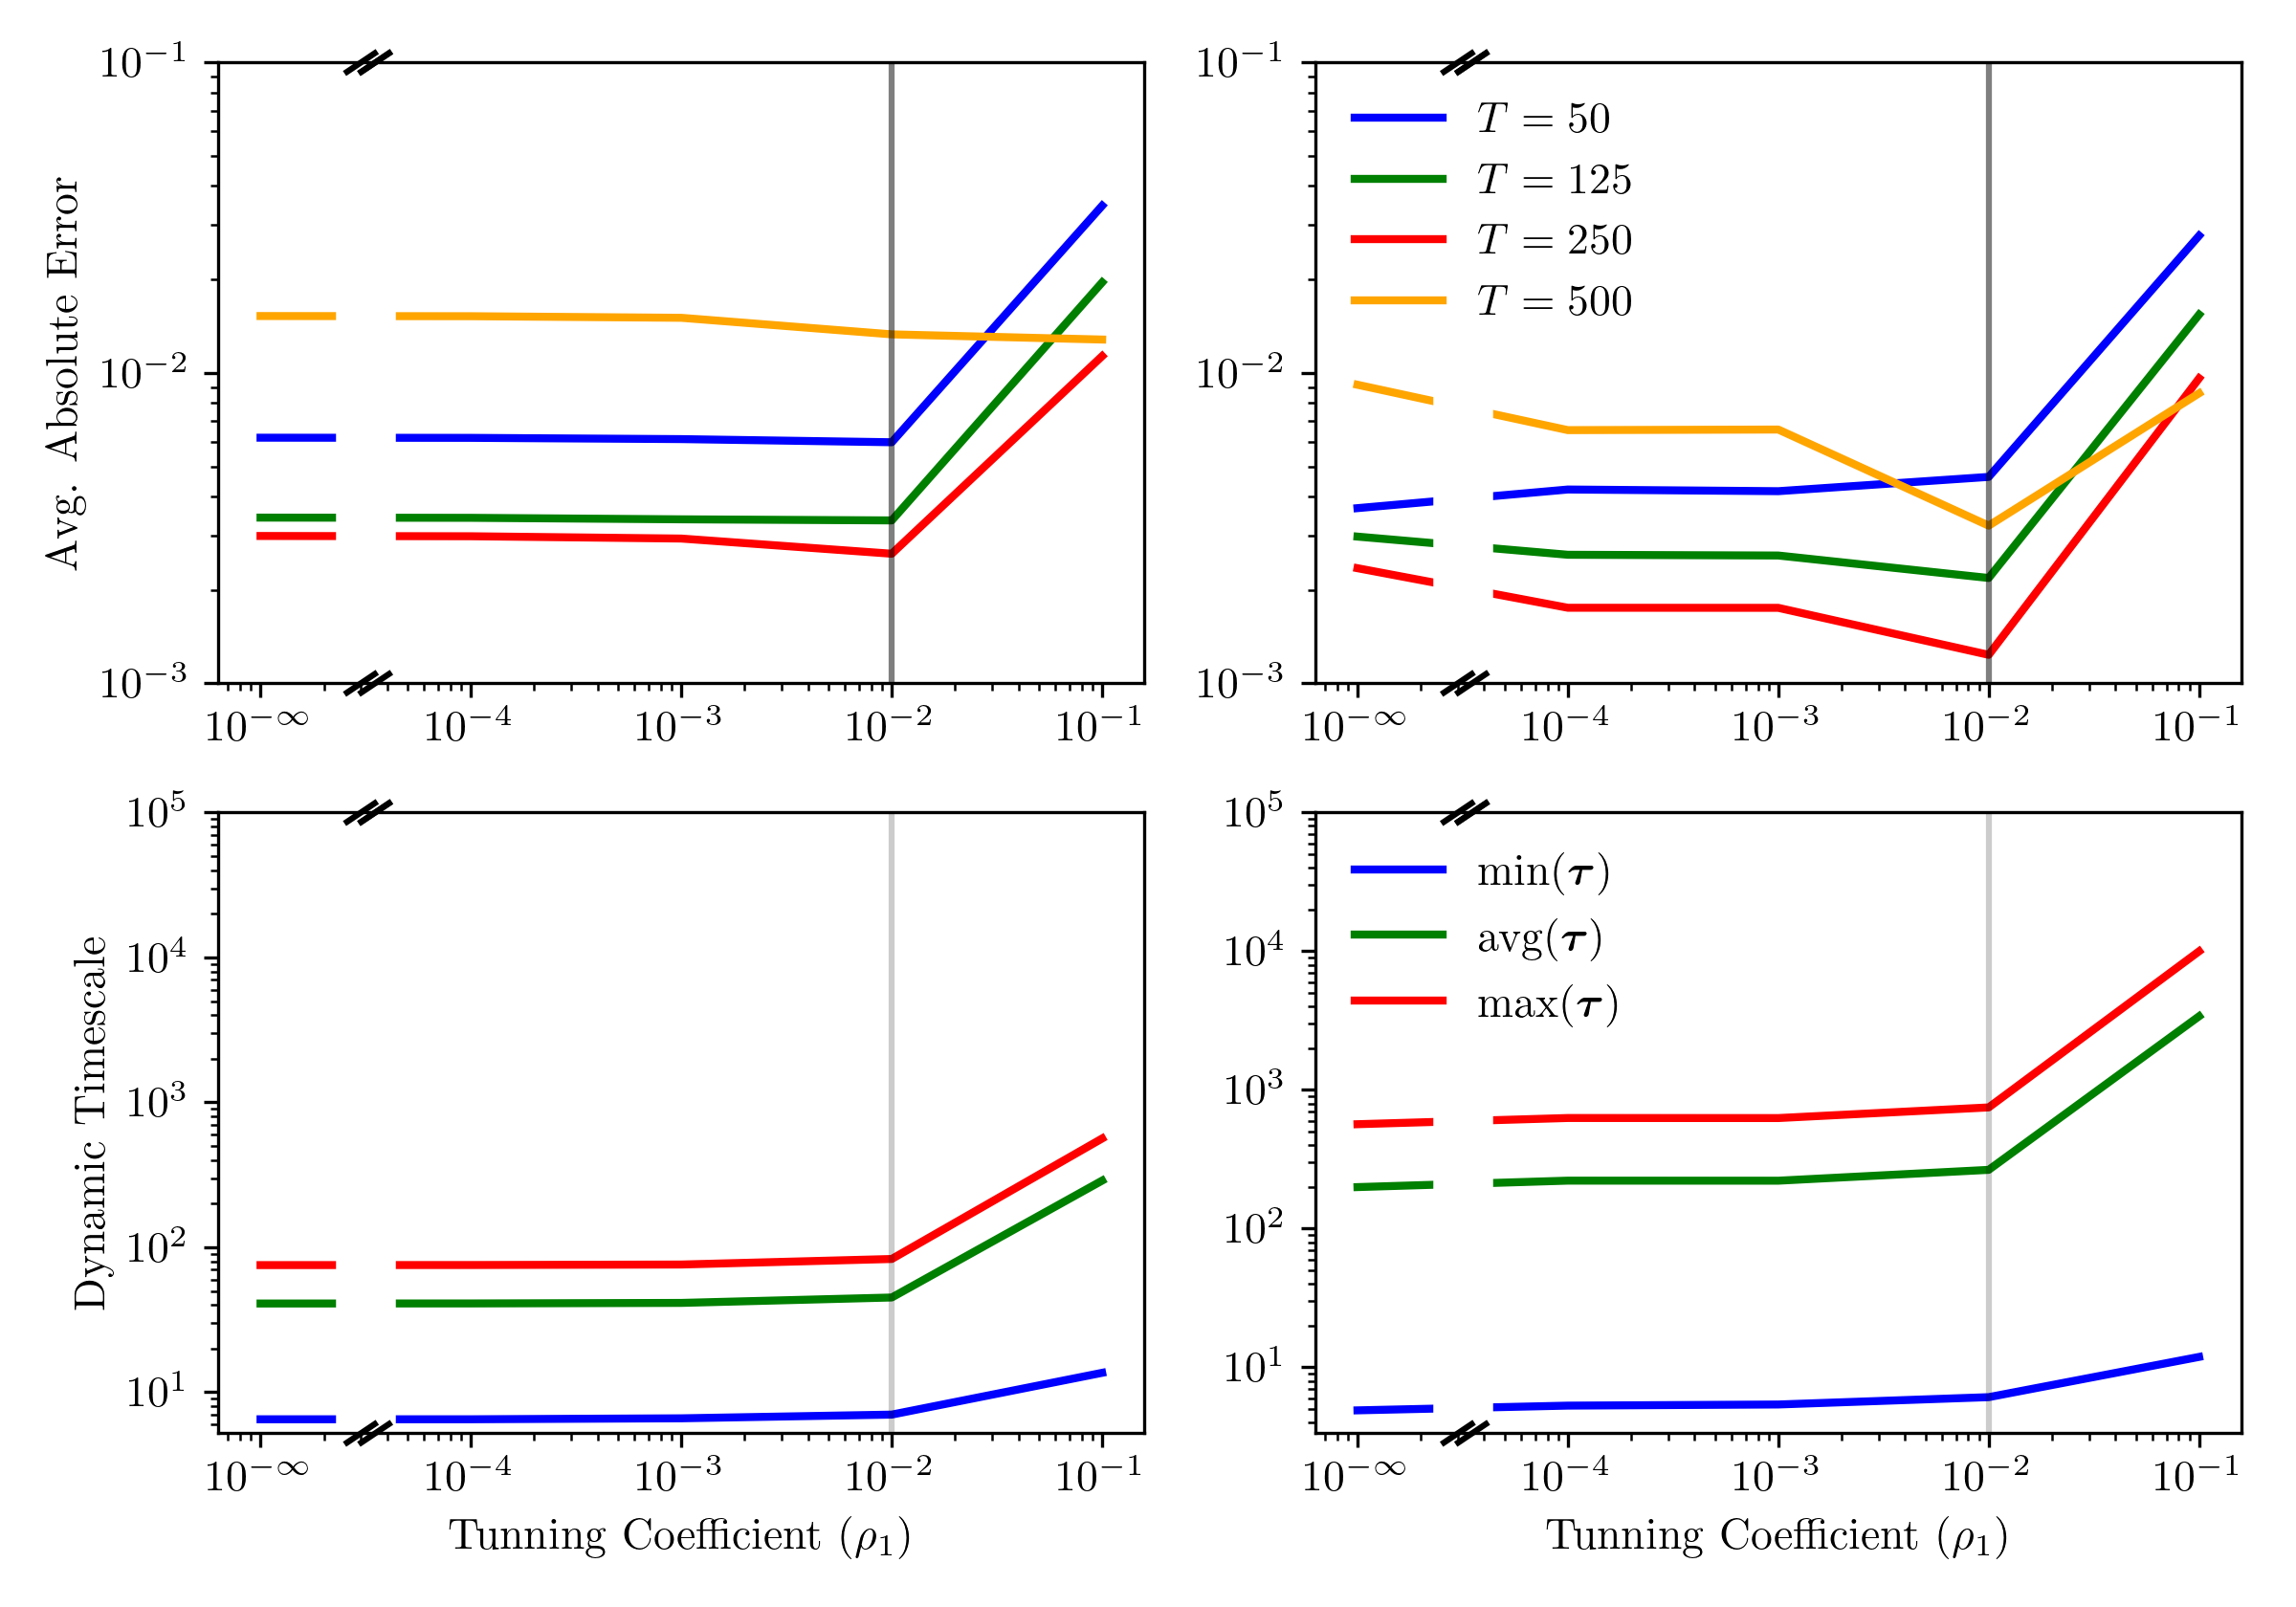
\includegraphics[width=\textwidth]{fig/analysis_rho_1_sel.png}
\caption{
The average absolute error and dynamic timescales $\bb{\tau}$ for the $3$SR (left-column) and $4$PR (right-column) model configuration for varying values of $\rho_1$ at fixed value of $\rho_2=\rho_3=\expnum{1}{-4}$.
%
The displayed error is calculated as the absolute difference between the emulator simulation and the $\mu$-benchmark, averaged  over a timespan of $T$ years following a $100$ GtC carbon pulse.
%
The black vertical line is the selected value $\rho_1=\expnum{1}{-2}$.
%
%Notice that $\rho_1=\expnum{1}{-\infty}$represents a test without the $q_1$ penalty function.  
}
\label{fig:rho_1_motiv}
\end{figure}

%
Here we outline the calibration results for the fitting procedure described in Section~\ref{sec:2.2}.
%
The minimization program in~\eqref{eq:obj} and ~\eqref{eq:objc} are carried out using a differential evolution optimizer~\cite{diff_evol}, as implemented in the SciPy Python package~\cite{scipy}.
%
In all tests conducted, we set $\bbt{m}_{\text{A}} = 586$ to represent the preindustrial atmospheric equilibrium condition, as cited in \cite{IPCC_carbon_cycle}. 
%
For both $3$SR and $4$PR model configuration, we fix the tuning coefficients $\rho_2=\rho_3=\expnum{1}{-4}$.
%
Note that for the $3$SR configuration, the $q_3$ penalty function in \eqref{eq:q3} which is associated with reservoir absorption ratios, has no influence as the model lacks a land-biosphere component.
%
In Figure~\ref{fig:penelty_motiv} we show the effect of the penalty function, or equivalent the tuning coefficients $\rho_1$, $\rho_2$ and $\rho_3$, on the solution dynamics.
%
Notability, setting either $\rho_2$ or $\rho_3$ to $\expnum{1}{-4}$ (while keeping $\rho_1=0$) results in minimal changes to the overall dynamics of the $3$SR model, but leads to a significant change in the cumulative flux absorption across various reservoirs in the $4$PR model.

In Figure~\ref{fig:rho_1_motiv} we show the average absolute error emulated atmospheric carbon contented in comparison to the $\mu$-benchmark and dynamic timescales, for varying values of $\rho_1$.
 %
 The $3$SR model shows minimal sensitivity to $\rho_1$, which is associated with the $q_1$ penalty function that encourages larger dynamic timescales.
%
However, in the $4$PR model, we observe improvements in the average absolute errors most time periods after the initial pulse, with the lowest errors found at $\rho_1=\expnum{1}{-2}$.
%
In both model configurations, increasing $\rho_1$ resulting larger dynamic times scales $\bb{\tau}$. 
%
The $3$SR model can only represent two dynamic timescales, corresponding to two nonzero eigenvalues, whereas the $4$PR model can represent three.
%
We note that the $3$SR model is not sufficiently versatile to accurately represent short, medium, and long-term timescales simultaneously. 
%
Instead, the model appears to capture short-term dynamics while averaging out medium and long-term behaviors.
%
Inline with most penalized methods, for very large values of the tuning parameter, we see an increase in error as the weight of the penalty function begins to outweigh the actual model fit error.
 %
 





The results of the optimization process can vary depending on the random seed used, the initial guess, the convergence tolerance, and in particular the tuning coefficients $\rho_1$, $\rho_2$ and $\rho_3$. 
%
The initial guess for the optimizer is set to the mean of the lower and upper search bounds for the parameters $\bb{a}^{\mu}$ and $\bbt{m}^{\mu}$, as discussed in Section~\ref{sec:2.2.1} and shown in Table~\ref{tab:1}.
%
This is achieved by setting the lower and upper bounds for $\bbt{m}_{\text{A}}$ to be identical.
%
The convergence tolerance for the optimizer is set to $\expnum{1}{-6}$ for all tests.
%
As illustrated in Figure~\ref{fig:penelty_motiv}, setting either $\rho_2$ or $\rho_3$ to  $\expnum{1}{-4}$ (while keeping $\rho_1=0$) results in minimal changes to the overall dynamics of the $3$SR model, but leads to a significant change in the cumulative flux absorption across various reservoirs in the $4$PR model.
%
This is expected because the $3$SR model has fewer degrees of freedom than the $4$PR configuration. 
%
This difference highlights the need for penalty methods to constrain the solution space in more complex models like the $4$PR configuration.









\begin{table}[t]
\centering
\small
\begin{tabular}{cccccccccc||cc}
& 
\multicolumn{9}{c}{\textsc{Fitted parameters values}} &  \\
&
	$\bb{a}^{\mu}_{\text{A}   \to \text{O}_1}$ & 
	$\bb{a}^{\mu}_{\text{O}_1 \to \text{O}_2}$ & 
	$\bb{a}^{\mu}_{\text{A}   \to \text{L}  }$ &
	$\bbt{m}^{\mu}_{\text{A}}$    &
	$\bbt{m}^{\mu}_{\text{O}_1}$  &
	$\bbt{m}^{\mu}_{\text{O}_2}$  &
	$\bbt{m}^{\mu}_{\text{L}}$   &
	$\bb{c}^{\mu^+}$ &
	$\bb{c}^{\mu^-}$ &
$\bb{m}_{\text{O}}^{t_e}/\bb{m}_{\text{L}}^{t_e} $ & 
$\bb{\tau}$
\\[4pt]
%
\toprule
\toprule
\textit{Lower}& $\expnum{1}{-6}$ & $\expnum{1}{-6}$  & $\expnum{1}{-6}$ & $589$ &  $\expnum{1}{-6}$    & $\expnum{1}{-6}$  & $\expnum{1}{-6}$ & $\expnum{1}{-6}$  & 1 &  &\\
\textbf{3SR} & $\num{0.0769405}$ & $\num{0.0109354}$ & - & $589$ & $714 $    & $1,272 $  & - & 0.475 & 2.456 & - & $7/83$ \\
\textbf{4PR} & $\num{0.0208104}$ & $\num{0.0025498}$ & $\num{0.0613352}$ & $589$ & $1,076$ & $37,103$ & $404 $ & 0.470 & 2.407 & $0.75$  & $6/42/748$  \\
\textit{Upper}&   $0.3$ & $0.3$ & $0.3$  & $589$ & $1,800$ & $74,200$ & $1,100$ & $1$ & $5$ &  &\\
\end{tabular}
\caption{
The table shows the fitted parameter values, ratio of ocean and land pulse absorption ($\bb{m}_{\text{O}}^{t_e}/\bb{m}_{\text{L}}^{t_e} $), and dynamic timescales ($\bb{\tau}$), based on tuning coefficients $\rho_1$, $\rho_2$, and $\rho_3$, with respective values $\expnum{1}{-2}$, $\expnum{1}{-4}$, and $0.0$ for the 3SR model, and $\expnum{1}{-2}$, $\expnum{1}{-4}$, and $\expnum{1}{-4}$ for the $4$PR model.
%
The ratio of ocean and land pulse absorption is measured at $t_e=20$.
%
Also shown are the ``lower'' and ``upper'' search bounds for the possible parameters values, see Section~\ref{sec:2.2} for further details.
%
Note that $\bb{m}_{\text{A}}$ is fixed at the preindustrial value of $589$ GtC.
}
\label{tab:1}
\end{table}
















 \begin{figure}[h]
    \centering
	\raggedleft{\hspace{12em}\small{\textsc{3SR}}} \raggedright{\hspace{18em}\small{\textsc{4PR}}} 
    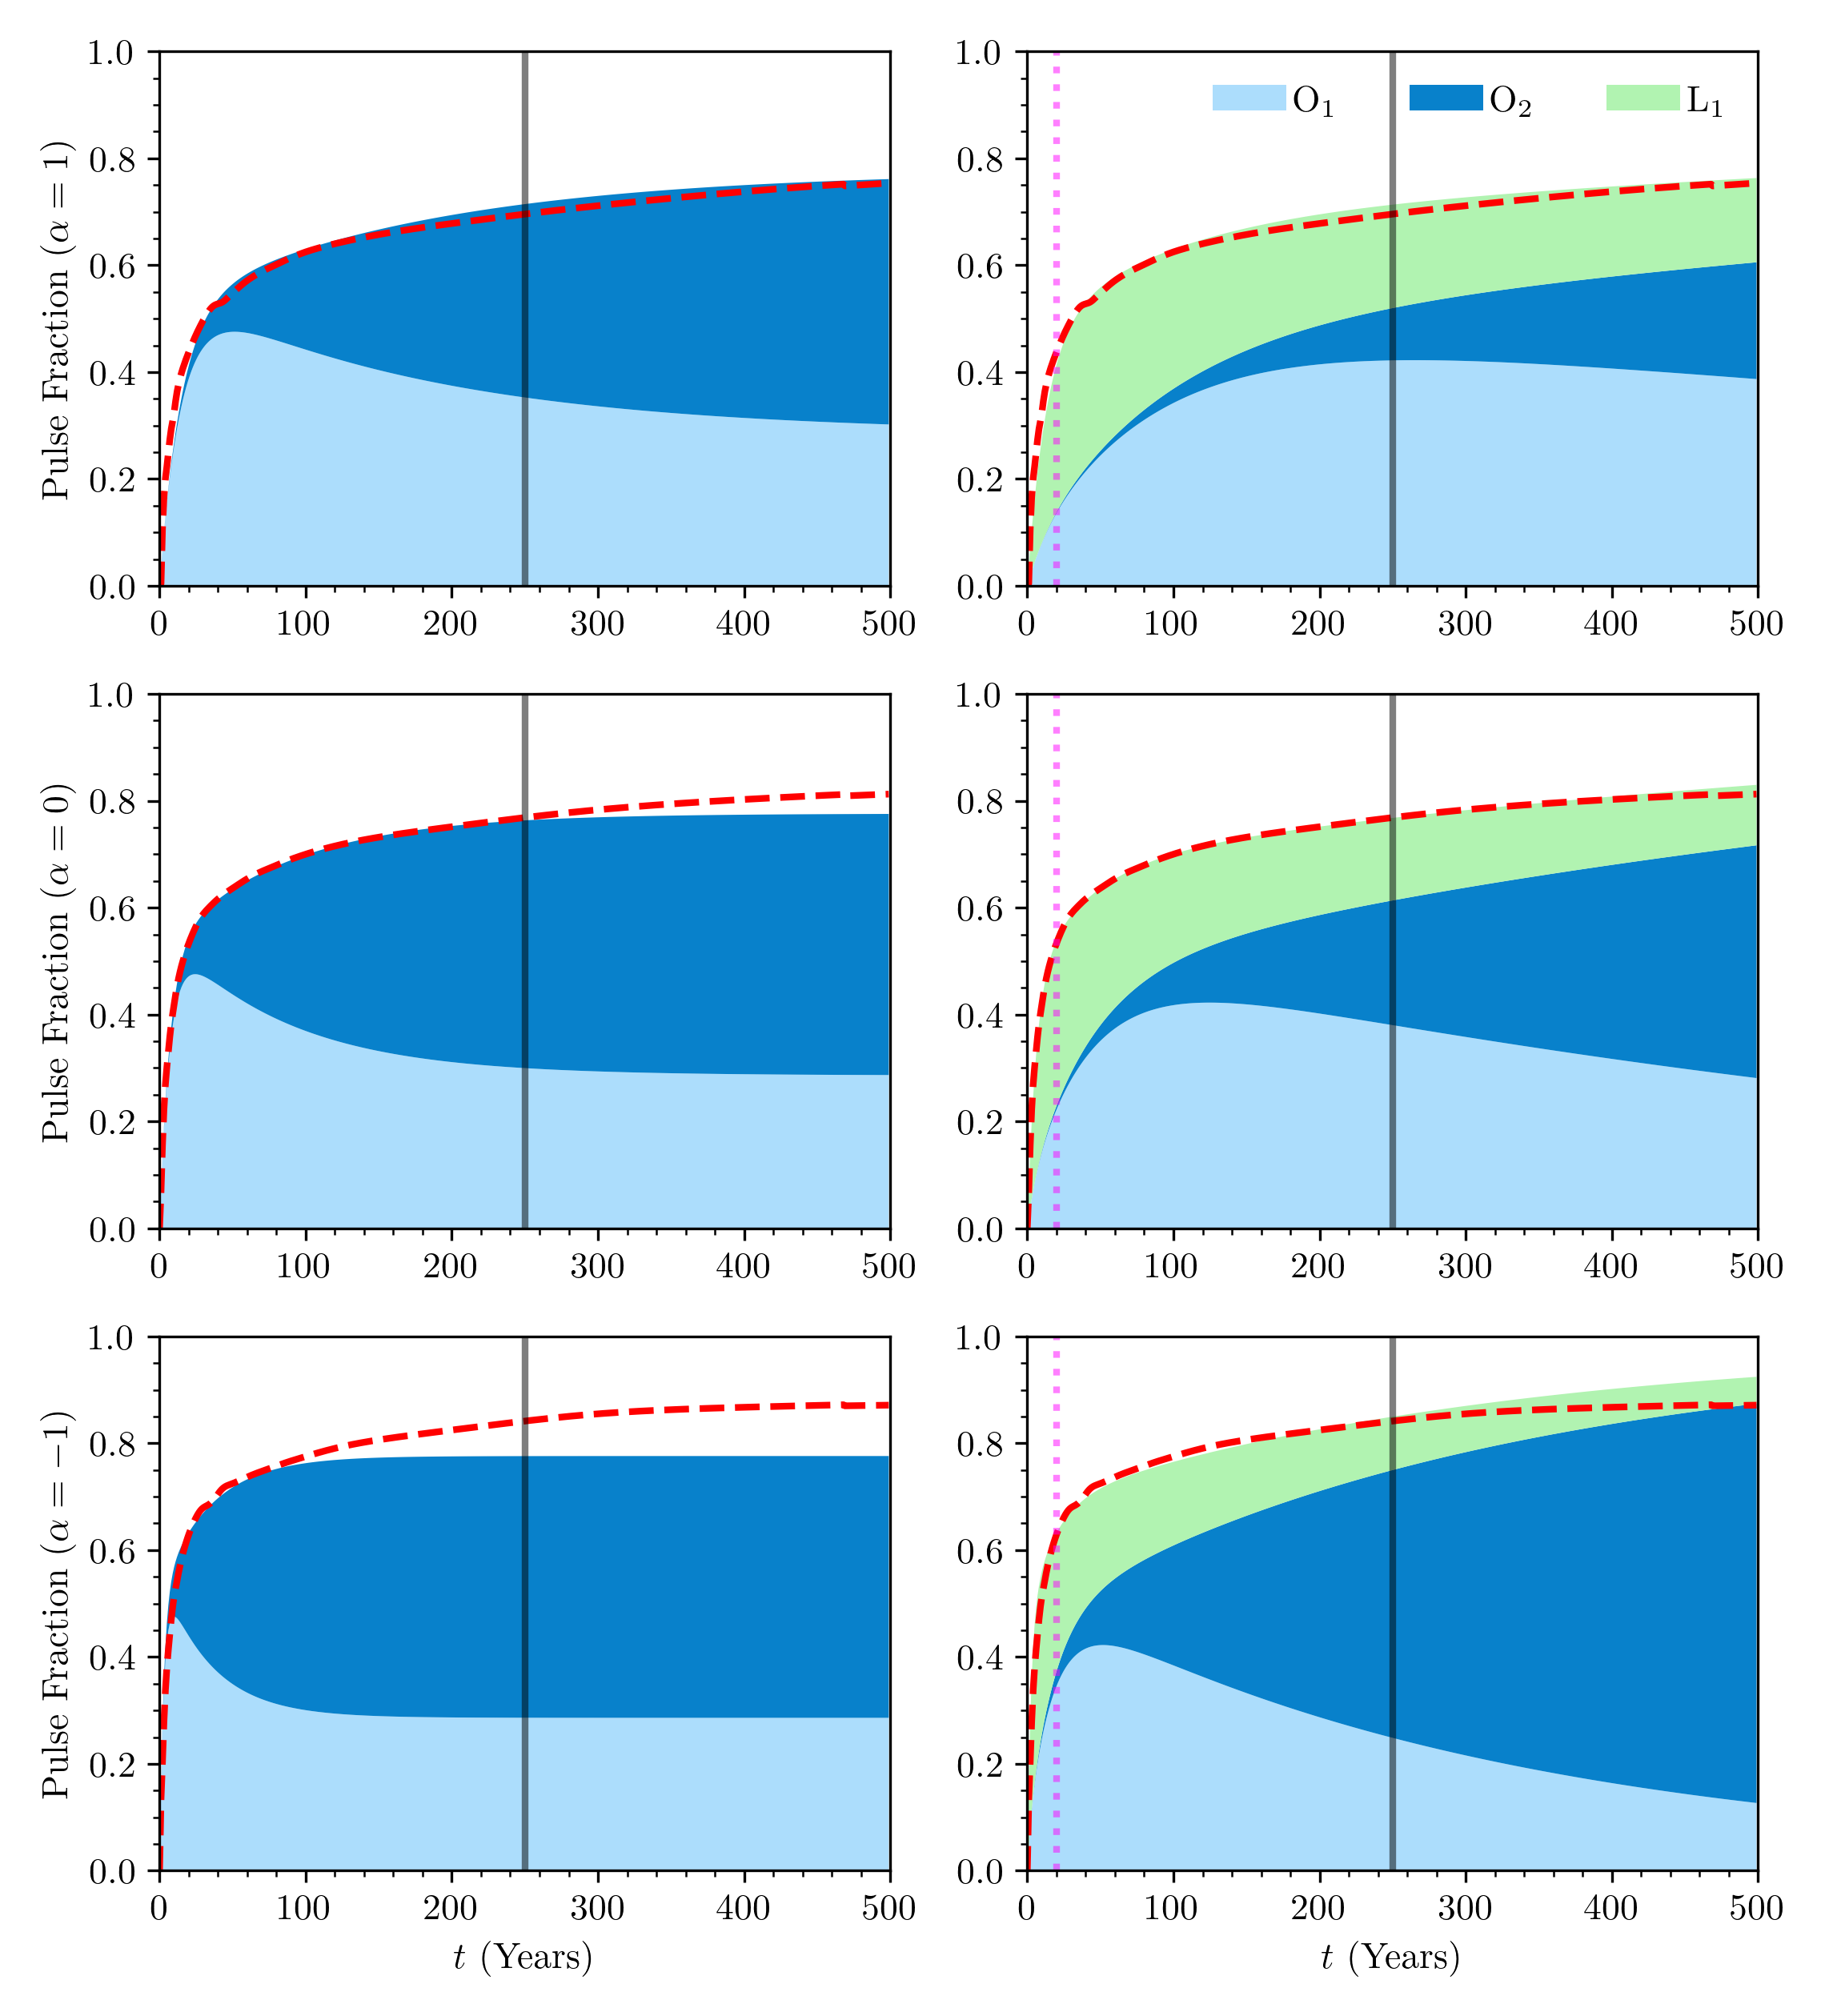
\includegraphics[width=\textwidth]{fig/plot_flux_alpha.png}
    \caption{
    The decay of a $100$ GtC pulse of emissions in the pre-industrial atmosphere (1765) was analyzed using various Earth System Models of differing complexities.
    This data is based on a series of controlled simulations conducted by~\cite{joos2013carbon}.
    %For further details on the simulations and model descriptions, we refer the reader to the cited reference. T
    The multimodal mean of the simulations, denoted by $\mu$, along with the two standard deviations above and below $\mu$-benchmark, are represented by $\mu^+$ and $\mu^-$, respectively.
     }
    \label{fig:fully_fitted}
\end{figure}
%
 
 
 
 

 \section{Simulations}
 
 
 
 
 \section{Pulse}
 
\begin{figure}[b]
    \centering
	\raggedleft{\hspace{12em}\small{\textsc{3SR}}} \raggedright{\hspace{18em}\small{\textsc{4PR}}} 
    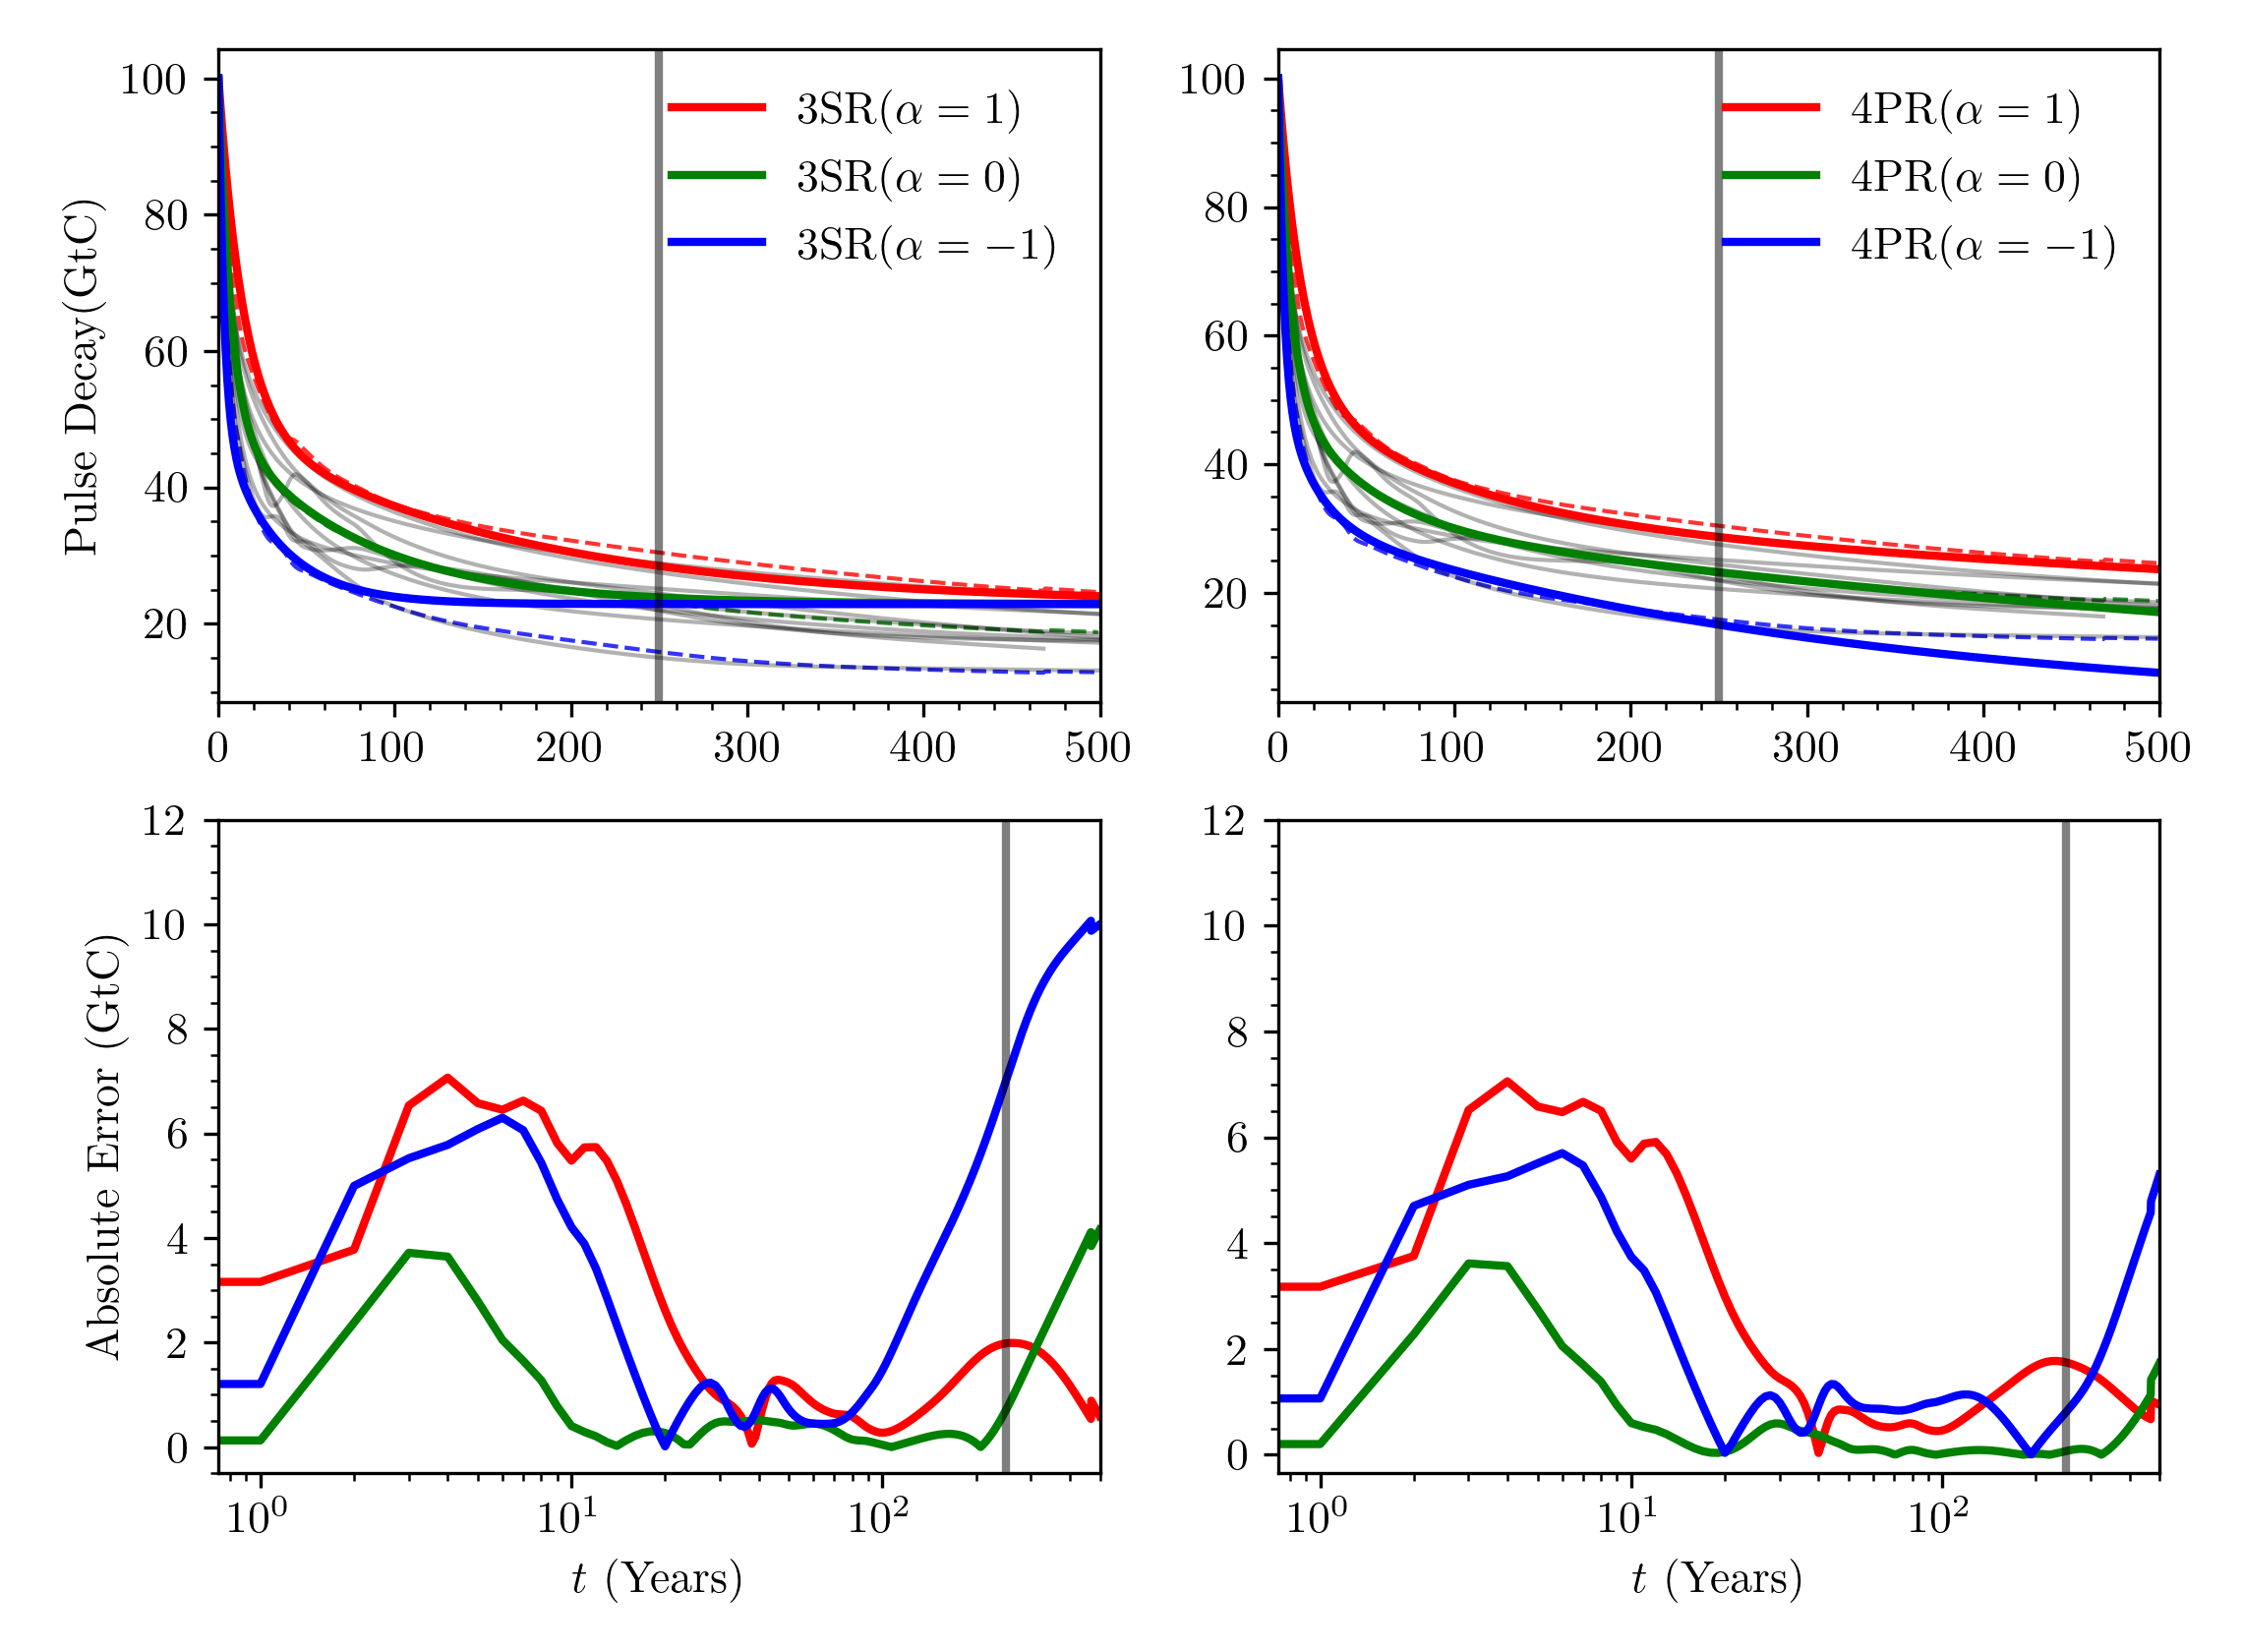
\includegraphics[width=\textwidth]{fig/plot_pulse_decay.png}
    \caption{
    DDD.
     }
    \label{fig:6}
\end{figure}
%


 
 
 \section{Pulse}
 
 
 
 


 

 

 
 

 
 
 
 












\clearpage
\newpage
\appendix
\section{Climate Emulator}
\addcontentsline{toc}{section}{Appendix}
%\setheader{Appendix}
\setcounter{figure}{0}                       % <---------------
\renewcommand\thefigure{A.\arabic{figure}}   % <---------------


%\section{Appendices}
\subsection{Coefficient Selection}
%
 \begin{figure}[t]
    \centering
	\raggedleft{\hspace{12em}\small{\textsc{3SR}}} \raggedright{\hspace{18em}\small{\textsc{4PR}}} 
    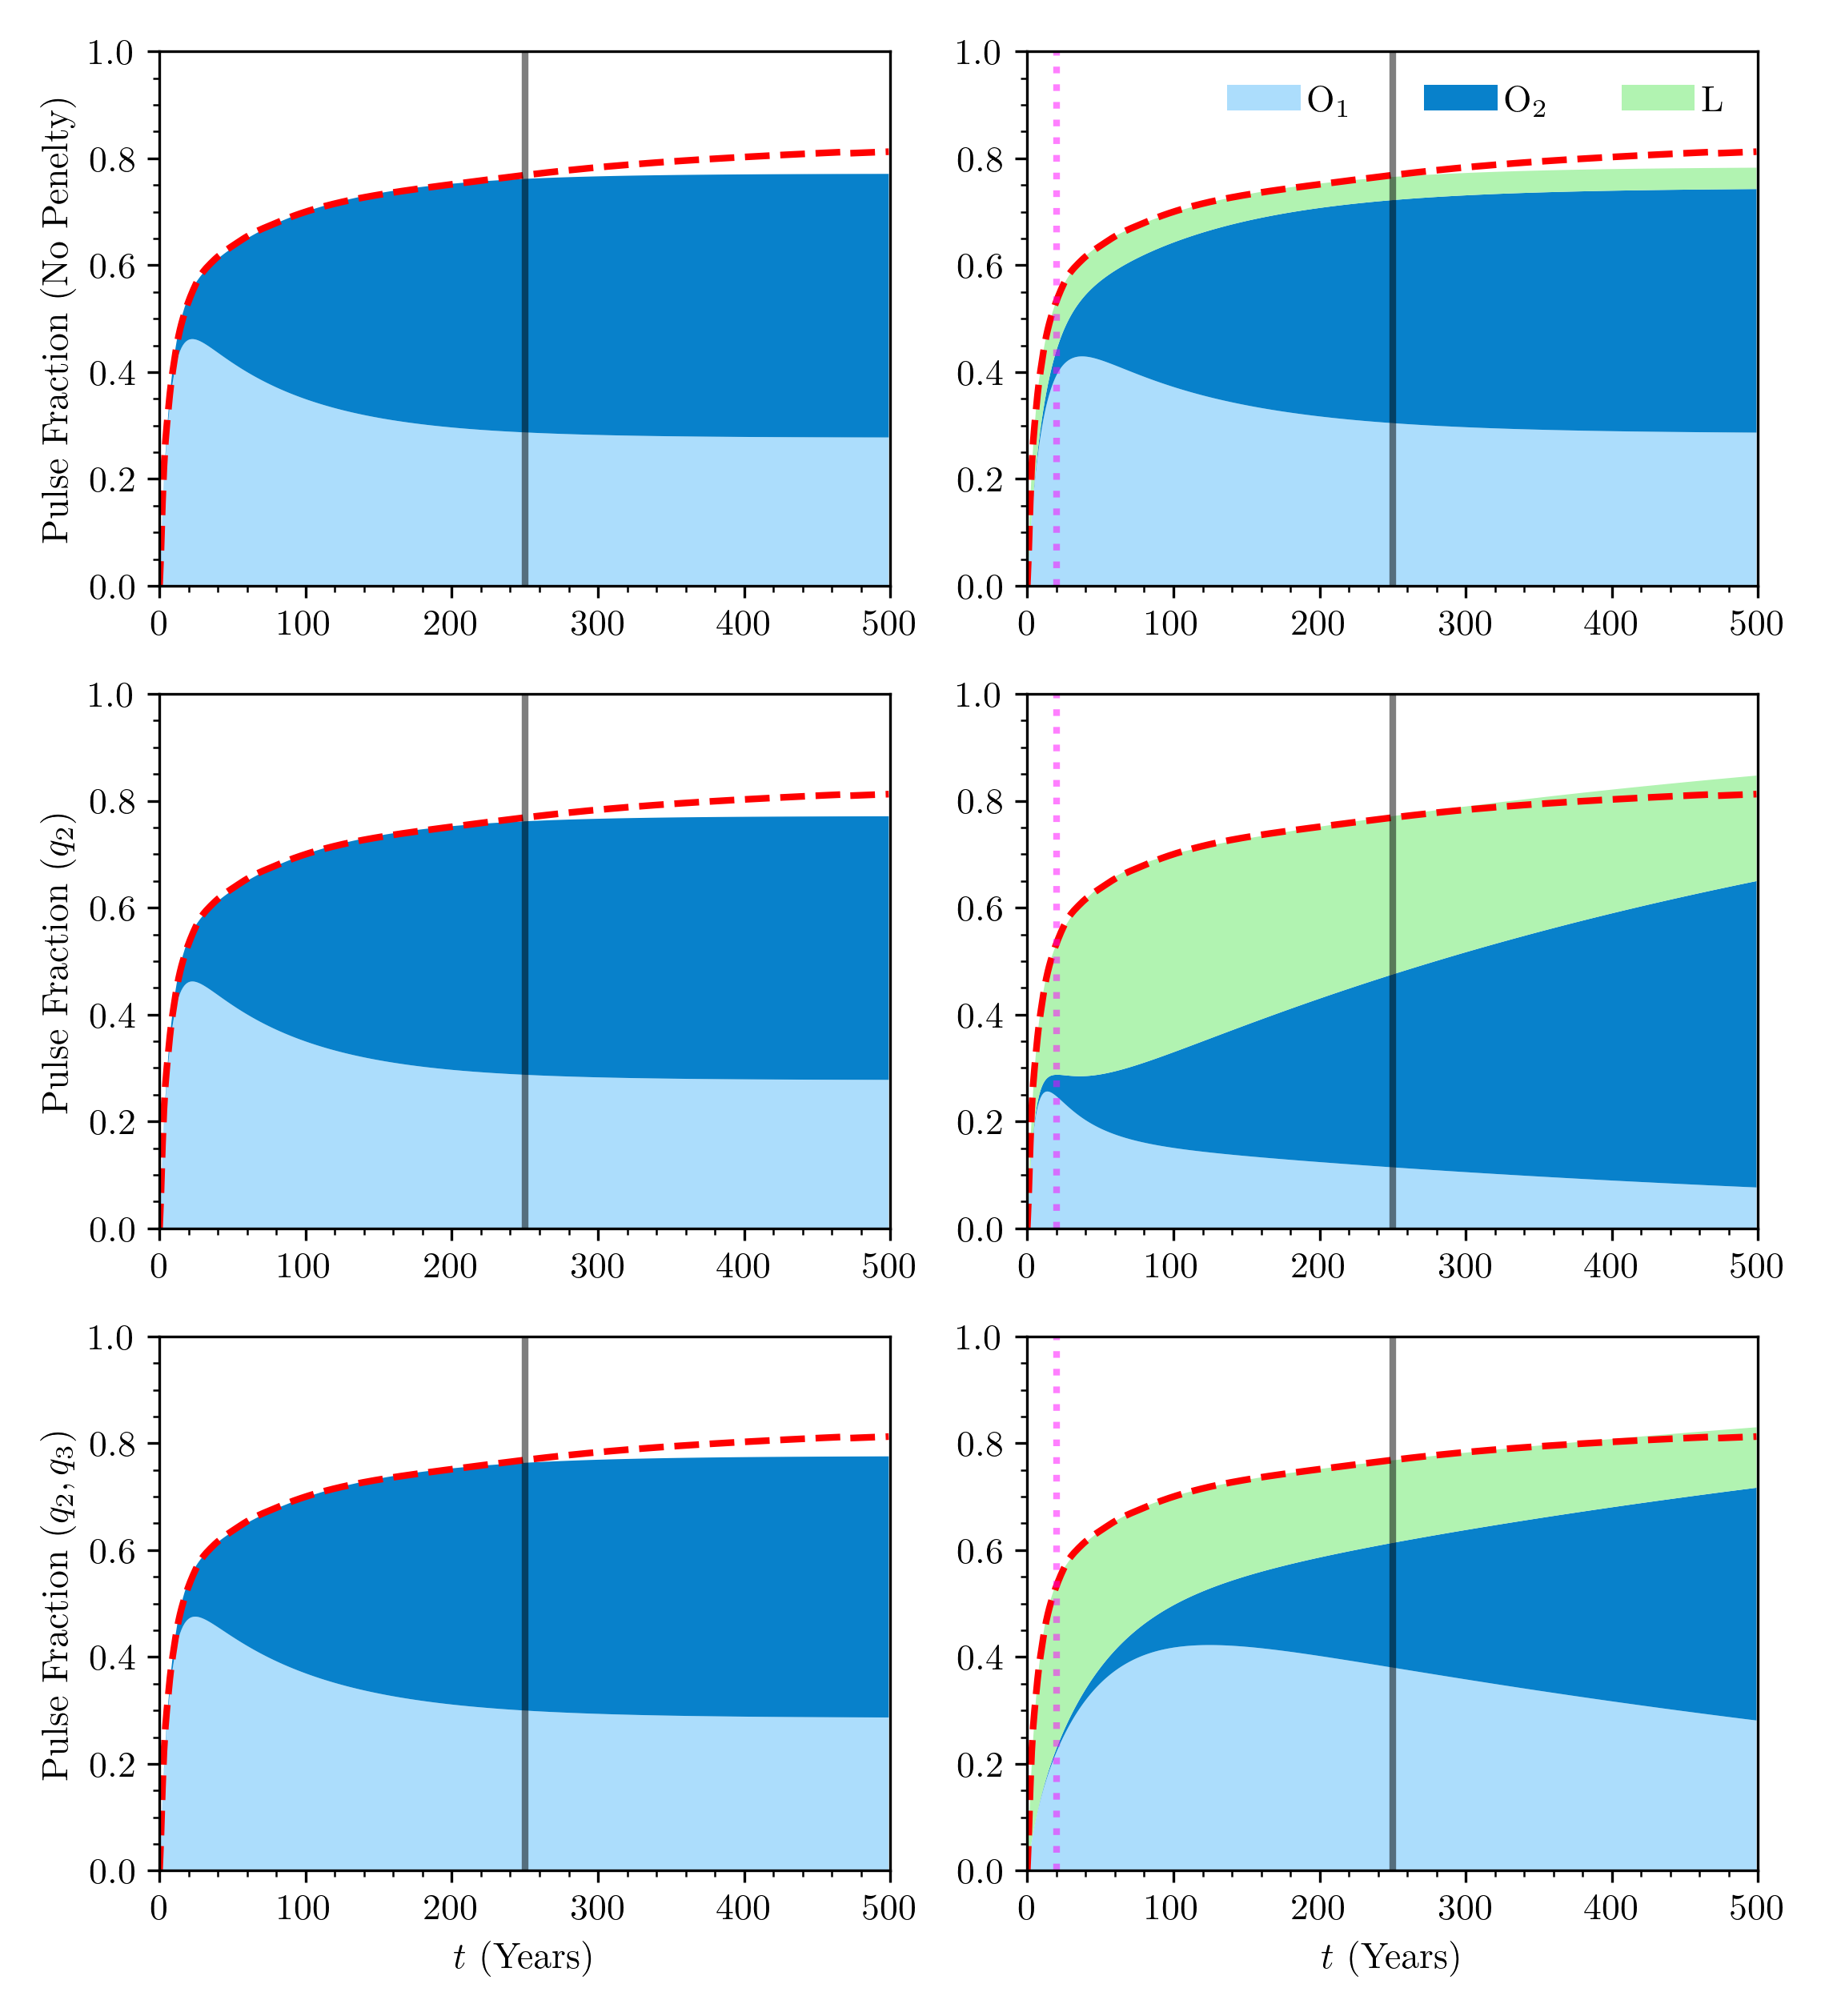
\includegraphics[width=\textwidth]{fig/plot_flux_pen.png}
    \caption{
    The decay of a $100$ GtC pulse of emissions in the pre-industrial atmosphere (1765) was analyzed using various Earth System Models of differing complexities.
    %
    This data is based on a series of controlled simulations conducted by~\cite{joos2013carbon}.
    %
    For further details on the simulations and model descriptions, we refer the reader to the cited reference.
    %
    The multimodal mean of the simulations, denoted by $\mu$, along with the two standard deviations above and below $\mu$-benchmark, are represented by $\mu^+$ and $\mu^-$, respectively.
     %
    The multimodal mean of the simulations, denoted by $\mu$, along with the two standard deviations above and below $\mu$-benchmark, are represented by $\mu^+$ and $\mu^-$, respectively.
      %
    The multimodal mean of the simulations, denoted by $\mu$, along with the two standard deviations above and below $\mu$-benchmark, are represented by $\mu^+$ and $\mu^-$, respectively.
     }
    \label{fig:penelty_motiv}
\end{figure}
%








 



\clearpage
% with BibTeX
\bibliography{references.bib}

\end{document}

%%% Local Variables:
%%% mode: latex
%%% TeX-master: t
%%% End: